%\IfFileExists{revtex4-1.cls}{\documentclass[prd, twocolumn, lengthcheck, superscriptaddress, showpacs, letterpaper, footinbib]{revtex4-1}}{ 
%\IfFileExists{revtex4.cls}{\documentclass[prd, twocolumn, lengthcheck, superscriptaddress, showpacs, letterpaper]{revtex4}}{}}
\documentclass[11pt,a4paper]{emulateapj}
\bibliographystyle{apj}

\usepackage{epsfig}
%\usepackage{amsmath}
\usepackage{natbib}

%\documentclass[prd, twocolumn, lengthcheck,superscriptaddress, showpacs, letterpaper, footinbib]{revtex4}
%\documentclass[lengthcheck,superscriptaddress,showpacs,letterpaper,nofootinbib]{article}
\usepackage{ifpdf}
\usepackage[bookmarks=false]{hyperref}
\pdfoutput=1
\usepackage[usenames,dvipsnames]{color}
\usepackage{graphicx}
\usepackage{graphics}  
  \usepackage{float}
%\restylefloat{table}
\usepackage{amsmath}
\usepackage{amssymb}
\usepackage{acronym}
\usepackage{comment}
\usepackage{multirow}
\usepackage{xspace}
%\restylefloat{figure}
\usepackage{units}
\usepackage{dcolumn}
\usepackage{ulem}

\def\aj{Astron. J.}                 % Astronomical Journal
\def\apj{Astrophys. J.}                % Astrophysical Journal
\def\apjl{Astrophys. J. Lett.}             % Astrophysical Journal, Letters
\def\pasj{PASJ}
\def\apjs{Astrophys. J., Suppl. Ser.}              % Astrophysical Journal, Supplement
\def\mnras{Mon. Not. R. Astron. Soc.}            % Monthly Notices of the RAS
\def\prd{Phys. Rev. D}       % Physical Review D
\def\prl{Phys. Rev. Lett.}    % Physical Review Letters
\def\cqg{Class. Quant. Grav.}%Classical and Quantum Gravity
\def\araa{Annu. Rev. Astron. Astrophys.}             % Annual Review of Astron and Astrophys
\def\nat{Nature}              % Nature
\def\aap{Astron. Astrophys.}                % Astronomy and
                                % Astrophysics
\def\jasa{J. Am. Stat. Assoc.}
\def\pccp{Phys. Chem. Chem. Phys.}
\def\jrssb{J. R. Stat. Soc. B}
\def\aipcs{AIP Conf. Ser.}
\def\jcp{J. Chem. Phys.}

\newcommand{\carl}[1]{{\color{red}  #1}}
\newcommand{\tyson}[1]{{\color{blue} #1}}
\newcommand{\ben}[1]{{\color{green} #1}}
\newcommand{\will}[1]{{\color{cyan} #1}}
\newcommand{\vivien}[1]{{\color{purple} #1}}
\newcommand{\diego}[1]{{\color{pink} #1}}

\newcommand{\thpara}{\boldsymbol{\theta}}
\newcommand{\chmass}{\mathcal{M}_c}



\begin{document}
\title{Basic Parameter estimation of Binary Neutron Star Systems by the Advanced LIGO/Virgo Network}
\author{Carl L. Rodriguez \altaffilmark{1}
%\email{rodriguez@u.northwestern.edu}
Benjamin Farr \altaffilmark{1}
%\email{bfarr@u.northwestern.edu} 
Vivien Raymond \altaffilmark{1,2}
Will M. Farr \altaffilmark{1}
%\email{w-farr@northwestern.edu} 
Tyson Littenberg\altaffilmark{1}
%\email{tyson.littenberg@northwestern.edu}
Diego Fazi\altaffilmark{1}
%\email{d-fazi@northwestern.edu}
Vicky Kalogera\altaffilmark{1}}
%\email{vicky@northwestern.edu}

\altaffiltext{1}{Center for Interdisciplinary Exploration and Research in Astrophysics (CIERA) \& Dept.~of Physics and Astronomy, Northwestern University, 2145 Sheridan Rd, Evanston, IL 60208, USA; [e-mail: {\tt cr@u.northwestern.edu}]}
\altaffiltext{2}{California Institute of Technology, Pasadena, CA 92215, USA}



\begin{abstract}

Within the next five years, the Advanced LIGO/Virgo network will have reached a sensitivity sufficient to enable the routine
 detection of gravitational waves.  Beyond the initial detection, the scientific promise of these instruments relies on the ability to perform parameter estimation. The majority of this effort has been towards the detection
   and characterization of gravitational waves from compact binary coalescence, e.g. the coalescence of binary 
   neutron stars.  While several previous studies have focused on the parameter estimation abilities of advanced detectors, 
   the majority have relied on approximation techniques such as the Fisher Matrix.  We report the statistical 
   uncertainties that will be achievable, in practice, using the full parameter estimation machinery developed by the  
   LIGO/Virgo Collaboration.  We find the recovery of the individual masses to be fractionally within 
   10\% at the 65\% credible intervals for equal-mass systems, and within 2\% for unequal-mass systems.
     We also report the average uncertainties on the sky-locations, luminosity distance, and orbital inclinations of randomly 
     distributed sources that can be achieved by different network configurations.
\end{abstract}

\maketitle
\section{Introduction}

Within the next few
 years, the first generation of gravitational-wave detectors capable 
 of regularly resolving astrophysical sources will come online \citep{AdvLIGO,AdvVirgo}.
 The Advanced LIGO and Virgo detectors will provide the first insights
 into the final moment of binary compact object mergers, including the 
 merger of binary neutron star systems.  Intense preparations are underway
 to characterize and extract as much physical 
 information as possible from these signals.
 
The mergers of binary neutron stars (BNS) are expected to be the most common
compact binary source in the advanced detector era.   Models from stellar 
evolution and observations of binary pulsars suggest that the number of binary neutron star mergers within 
Advanced LIGO/Virgo's detection horizon could reach into the hundreds each 
year, with an expected mean of $\sim 40$ per year \citep{RatesPaper}. 
Although the peak sensitivity of ground-based detectors
is not focused on the frequency at which BNS systems merge, it could still
be possible to extract information about both strong field gravitational 
physics \carl{[CITE]} and the hydrodynamics of dense matter (e.g. the equation 
of state of nuclear matter) \carl{[CITE]}.  Furthermore, the observations of multiple BNS
systems will provide key insight into the evolution of binary systems in the field \citep{VickyRates,KimRates}
. As such, BNS systems will likely 
form the ``bread and butter'' of the compact binary coalescence detection effort in the coming 
years.


Of course one must distinguish between the detection of 
such events, and the precision measurement of the relevant physical parameters.
The detection of BNS systems will be performed with a matched filtering approach.  
By comparing the data stream with a bank of theoretical templates, the 
 time-series data can be searched for candidate signals at a sufficiently
  rapid rate to analyze months of data.  When the overlap between one of the template waveforms and the 
detector output is sufficiently large (97\%), a detection candidate is found.  However,
the parameter space of these signals can be highly degenerate, with several 
locations in parameter space corresponding to nearly identical waveforms.  In 
order to fully realize the science potential of these instruments, we must 
perform a full exploration of the parameter space for each detection.  By 
analyzing the parameter space of each candidate with a Bayesian inference technique, 
 we will be able to make precise, scientifically meaningful
statements about the physics of these systems.  To 
that end, we employ a Markov-Chain Monte Carlo sampling algorithm, 
\texttt{lalinference\_mcmc}, included in the LIGO Application Library parameter
estimation code, \texttt{LALInference}, to analyze the parameter space of BNS systems.

By employing the full parameter-estimation machinery that will eventually be
used in the Advanced LIGO/Virgo era, our results give the first estimates at the 
realistic capabilities of advanced ground-based detectors to characterize BNS systems.
  Until recently, the majority of studies have employed the Fisher matrix formalism which was 
first adapted for gravitational-wave parameter estimation by \citep{FinnDetection}.
While each of these studies \citep{PoissonWill,CutlerFlanagan,ArunPE} have pointed out the limitations 
and flaws of the Fisher Information Matrix, there has been no study which investigates
the BNS parameter estimation capabilities of Advanced LIGO/Virgo using the techniques
that will eventually be employed.  The recent work of \cite{Vallisneri} and our 
own work \citep{Inadequacies} has demonstrated that the Fisher matrix cannot even
be treated as a lower bound on the standard deviations of certain parameters
(particularly the masses) measurable in gravitational-wave detectors.

In this paper, we perform a systematic study of the statistical uncertainties with
which the Advanced LIGO/Virgo network will be able to measure the basic parameters of 
BNS mergers.  In Section \ref{PEsection}, we describe
the machinery of our parameter estimation code, \texttt{LALInference}, and the associated
MCMC sampler, \texttt{lalinference\_mcmc}, as well as the frequency-domain 
gravitational-wave template we employ.   In Section \ref{resultsSection}, we qualitatively 
analyze the posterior probability density functions for BNS systems with different masses 
and extrinsic parameters.  The results are divided into three parameter sets of interest: the
recovery of the mass parameters (Section \ref{massSection}), the recovery of the orbital
inclination and luminosity distance (Section \ref{idSection}), and the localization of sources 
on the sky (Section \ref{skySection}).   Finally we provide quantitative 1-dimensional confidence
 intervals on each parameter in Section \ref{ciSection}.  These results, contained
 in Tables \ref{ciTableIntrinsic} and \ref{ciTableExtrinsic}, are intended as a reference for the 
 optimal BNS parameter estimation capabilities of Advanced LIGO/Virgo.
   We assume that $G=c=1$ throughout.


\section{Parameter Estimation}
\label{PEsection}


We begin by introducing a Bayesian formalism for parameter estimation. 
%Before offering a brief derivation of the FIM, a few preliminary
%techniques must be introduced.  First,
We assume that the time-domain signal in a gravitational-wave
network can be written as a combination of a gravitational
waveform $h_0$ and the noise of the detector $n$.  We further assume
that this noise is stationary and Gaussian with zero mean.  Therefore,
the detector output is simply
\begin{equation}
s = n + h_0 .
\label{SignalAddition}
\end{equation}
Since the noise model is Gaussian, we can write the
probability of a specific signal realization $s$ as proportional to the probability
that the residual is Gaussian distributed once the waveform has been subtracted
\begin{align}
  p(s | \thpara) &\propto \exp\left[-\frac{1}{2}\left<n|n
    \right>\right] \nonumber \\ &= \exp\left[-\frac{1}{2}\left < s -
    h(\thpara) | s-h(\thpara)\right >\right] ,
  \label{likelihood}
\end{align}
where $\thpara$ is the set of parameters for the template
waveforms, and $p(s | \thpara)$ is the likelihood of the signal $s$ given the parameters $\thpara$.
  The inner product, $\left< ~|~ \right> $, is defined using the noise
spectrum of the detectors as
\begin{equation}
  \left<a|b\right> \equiv 4 \Re \int \frac{\tilde{a}(f)\tilde{b}^*(f)}{S_n(f)} df ,
  \label{innerProduct}
\end{equation}
where $S_n(f)$ is the one-sided power spectral density (PSD) as a function
of frequency, and $\tilde{a}(f)$ and $\tilde{b}(f)$ are the Fourier
transforms of the time-domain data $a(t)$ and $b(t)$.  If we pick a set of parameters $\thpara$ such that
$h(\thpara) = h_0$, then the posterior \eqref{posterior}
will be near a global maximum; however, the presence of noise will in
general deflect the maximum of our posterior away from the value at
$\thpara_0$. That is, in the presence of noise, there is
no guarantee that the maximum-likelihood of our signal corresponds to
the true parameters of the system. 
 
Once we have the likelihood of the signal \eqref{likelihood}, we
employ Bayes Theorem to obtain the posterior probability of the system
parameters $\thpara$ given the signal $s$ as
\begin{align}
  p(\thpara | s) &= \frac{p(\thpara)p(s | \thpara)}{p(s)} \nonumber\\
  & \propto p(\thpara) \exp\left[-\frac{1}{2}\big < s - h(\thpara) | s-h(\thpara) \big > \right] ,
  \label{posterior}
\end{align}
where $p(\thpara)$ are the prior probabilities on our
source parameters and $p(s)$ is a normalization constant.

We are interested in the posterior $p(\thpara | s)$ as it encodes information about the
prior state of knowledge about the problem in addition to the likelihood of the signal.
  For instance, since it is assumed that compact binaries
form homogeneously in the local universe observable by advanced detectors,
 we can safely assume that the population of
sources will be distributed homogeneously in volume, or evenly in $D^2$. 
 Our prior information can come from mathematical limits in the parameter space or
from our \textit{a priori} knowledge of astrophysical systems.  We employ priors which are

\begin{itemize}
\item uniform in component masses from $0.8M_{\odot} \leq M_{1,2} \leq 30M_{\odot}$, with a minimum chirp mass  \eqref{eqRatioCM} of 0.6 $M_{\odot}$,
\item uniform in volume, which implies a luminosity distance prior of $p(D) = D^2 dD$, and
\item uniform in all other parameters.
\end{itemize}

\noindent  The mass priors listed here are the generic priors used in follow-up analysis, not specifically for BNS systems.  While we could have used a prior with a lower component mass cutoff for the present study, in practice the higher prior boundary does not effect our current analysis.


  
\subsection{Markov-Chain Monte Carlo}
\label{MCMCSection}
  
The LIGO Algorithm Library Bayesian inference code, \texttt{LALInference}, is designed as 
a unified framework for gravitational-wave parameter estimation.  By using a common setup for 
waveform generation, PSD estimation, data handling, and other associated techniques from gravitational-wave parameter estimation, \texttt{LALInference} allows the implementation of multiple samplers of the parameter space, including Nested Sampling (\texttt{lalinference\_nest}, described in \cite{nestedsampling2010}) and Markov-Chain Monte Carlo (\texttt{lalinference\_mcmc}).  We elect to use the MCMC sampler for this study.  \texttt{lalinference\_mcmc} is based upon the previously described code, 
\texttt{SpinSpiral} \citep{spinspiral2009, spinspiral2010}.  The MCMC employs a Metropolis-Hastings sampling algorithm, which can be described as follows \citep{Gilks99}:
  
\begin{enumerate}
\item Pick an initial point in the parameter space
  ($\boldsymbol{\theta_{\text{old}}}$), and then propose a random
  ``jump'' to a new set of waveform parameters,
  $\boldsymbol{\theta_{\text{new}}}$.  The jump follows the
  (conditional) probability distribution $q\left(
  \boldsymbol{\theta_{\text{new}}} | \boldsymbol{\theta_{\text{old}}}
  \right)$.
\item Calculate the posterior probability,
  $p(\boldsymbol{\theta_{\text{new}}}|s)$, of the new parameters using
  \eqref{likelihood} and \eqref{posterior}.
\item Accept the new parameters with probability 
  \begin{equation}
    p_\mathrm{accept} = \min \left[ 1, \frac{p(\boldsymbol{\theta_{\text{new}}}|s) q\left(\boldsymbol{\theta_{\text{old}}} | \boldsymbol{\theta_{\text{new}}} \right)}{p(\boldsymbol{\theta_{\text{old}}}|s) q\left(\boldsymbol{\theta_{\text{new}}} | \boldsymbol{\theta_{\text{old}}} \right)} \right].
  \end{equation}
  If the new parameters are accepted, record
  $\boldsymbol{\theta_\text{new}}$ and repeat with
  $\boldsymbol{\theta_\text{old}} \gets
  \boldsymbol{\theta_\text{new}}$; otherwise, record
  $\boldsymbol{\theta_\text{old}}$, and repeat.
\end{enumerate} 
  
The above procedure is designed to record a chain of samples whose
distribution is $p\left(\thpara|s\right)$.  By drawing a sufficient ($\sim1000$) number
 of effectively independent samples from the posterior, the chains traces out the functional form of the posterior,
 gathering more samples from regions with high posterior probability density.  Depending on
the proposal distribution, $q$, the convergence (mixing) of the chain
may be rapid or slow.  We employ multiple optimization techniques,
including both specially-crafted jump proposals ($q$) and parallel tempering, to ensure
adequate mixing of the Markov Chains throughout our parameter space.
Both samplers were tuned and 
developed during the last science run of the Initial LIGO/Virgo network.  
A description of the parameter estimation capabilities of these two samplers with respect to
real interferometer data, as well as a more detailed description of the algorithms and
checks for convergence, can be found in \cite{S6PE}.
  
 
\subsection{Waveform Model}
\label{waveformSection}
  
We use a frequency-domain waveform accurate up to $3.5$
post-Newtonian (pN) order in phase and 3 pN order in amplitude.  We restrict ourselves to
quasi-circular, non-spinning waveforms as a simplifying assumption.  The standard
form of our waveform model, known as the \textit{TaylorF2}
approximant, is calculated via the stationary-phase approximation.
  In this setup, the gravitational-wave
amplitude is given by
\begin{equation}
\tilde{h}(f) = a(t_f) e^{i \psi(f)},
\label{amplitude}
\end{equation}
where $a(t_f)$ is the amplitude evaluated at a stationary-phase reference point, which to lowest order
takes the form $a(t_f) \propto f^{-7/6} \chmass^{5/6}\Theta(\text{angle})/D$, where $D$ is
the luminosity distance of the binary, and $\psi(f)$ is the pN phase.
$\Theta(\text{angle})$ is a function of the orbital orientation with
respect to the detector network in terms of the sky position, orbital
inclination, and the wave polarization.  In addition to the total
mass, $M_{tot}\equiv M_1+M_2$, it is convenient to work with the
mass ratio and chirp mass, defined by
\begin{equation}
  q\equiv M_1/M_2~~~~\text{and}~~~~\chmass = (M_1 M_2)^{3/5} M_{tot}^{-1/5},
  \label{eqRatioCM}
\end{equation}
respectively.\footnote{Most gravitational-wave literature instead uses the \textit{symmetric mass ratio}, defined as $\eta \equiv M_1 M_2 / M^2$.  We elect to use $q$ as it is more physically intuitive, and the prior $p(q)$ is uniform when the component
mass priors are uniform.}  By convention, $M_1 \geq M_2$.  The stationary phase then becomes an expansion in the 
Newtonian orbital velocity, $v=(\pi M_{tot} f)^{1/3}$, 
\begin{equation}
\psi(f) = 2 \pi f t_c - \phi_0 + \frac{\pi}{4} + \frac{3}{128}\left(\frac{M_{tot}}{\chmass}\right)^{5/3}\sum^{n}_{k=0}\alpha_{k}v^{k-5}
\label{phase}
\end{equation}

\noindent where the $\alpha_{k}$ coefficients are taken from the pN expansion to order $n/2$.  See \cite{BuonannoWaveform} for a description and comparison of different waveform families.  The terms $t_c$ and $\phi_0$ in equation (\ref{phase}) are constants of integration, referred to as the chirp time and coalescence phase, respectively. 

To perform the integral defined in \eqref{innerProduct}, we used as our power-spectral
density the best estimate for a high-power, zero-detuning configuration of Advanced 
LIGO, provided by the LIGO Scientific Collaboration.  Both the noise curve and technical 
reports describing it can be found in \cite{ADVLIGONoise}.
We consider two configurations of the advanced detector
network: a three-detector configuation consistanting of the two LIGO sites 
(in Hanford, WA and Livingston, LA) and the Virgo site (in Pisa, Italy), and a 
four-detector configuration that adds the proposed LIGO-India detector
(in Chitradurga, KA).  For simplicity, we assume each detector to be 
operating at the Advanced LIGO sensitivity. 


For a multi-detector network, the noise-weighted inner products
\eqref{innerProduct} combine linearly, allowing us to use the above
formalism with minimal modification.  We integrate the inner product
from a lower-frequency cutoff of $20\text{Hz}$ to the
innermost-stable-circular orbit of the systems in question, which for a
non-spinning binary is a function only of the total mass:

\begin{equation}
  \pi f_{\text{ISCO}} = \frac{1}{6^{3/2}M_{tot}}.
  \label{ISCOFrequency}
\end{equation}
   
We consier the mass parameters ($\chmass,q$) and the phasing parameters,
($\phi_0,t_c$), to be the intrinsic parameters of a gravitational-wave signal.  There 
are an additional 5 extrinsic parameters, independent of the pN orbital phase, which can
modulate the amplitude of the signal in an independent fashion for each detector.  
Combining these leads to our 9-dimensional parameter space for non-spinning systems,
\begin{equation}
\thpara =  (\chmass, q, \phi_0,t_c,D,\iota,\psi,\alpha,\delta),
\label{parameterspace}
\end{equation}
where 

\begin{itemize}
\item $\chmass$ is the chirp mass,
\item $q$ is the mass ratio,
\item $\phi_0$ and $t_c$ are the chirp phase and chirp time, arbitrary phasing parameters,
\item $D$ is the luminosity distance to the binary,
\item $\iota$ is the orbital inclination (the angle between the orbital angular momentum and the line of sight), 
\item $\psi$ is the gravitational-wave polarization, and
\item $\alpha$ and $\delta$ are the right ascension and declination of the
source on the sky.
\end{itemize}
  Since the wave amplitude depends on the orientation of the
binary with respect to each detector, most of the information about these extrinsic
parameters comes from two quantities: the time-of-arrival triangulation of 
the source locations, and the relative amplitudes within the detector network.

We define the signal-to-noise ratio (SNR) of a gravitational wave in a
single detector as 
\begin{equation}
  \rho \equiv \frac{4}{\sigma} \int^{\infty}_{0}\frac{| \tilde{s}(f)\tilde{h}(f)|}{S_{n}(f)}df,
  \label{formalSNR}
\end{equation}
where $\rho$ is the SNR and $\tilde s(f)$ and $\tilde{h}^{*}(f)$ are
the frequency-domain data and template, respectively, and the normalization $\sigma$ is
given by
\begin{equation}
  \sigma^2 = 4\int^{\infty}_{0}\frac{| \tilde{h}(f)|^2}{S_n(f)}df.
  \label{SNRnorm}
\end{equation}

When dealing with network a of gravitational-wave detectors, the SNRs of the individual detectors add in quadrature.  That is, the network SNR for a detection is

\begin{equation}
\rho_{\text{network}} = \sqrt{\sum_i \rho_{i}^2}
\label{SNRnetwork}
\end{equation}

\noindent where $\rho_i$ is the SNR, given by \eqref{formalSNR}, of the $i^{\text{th}}$ detector.

For this study, we consider four seperate populations of BNS systems, with component mass 
combinations of $1M_{\odot}/1M_{\odot}$, $1.4M_{\odot}/1.4M_{\odot}$, $1M_{\odot}/2.5M_{\odot}$, 
and $2.5M_{\odot}/2.5M_{\odot}$.  Each population consisted of 40 signals distributed randomly
in sky location, polarization, inclination, time-of-arrival, and coalescence phase.  The luminosity 
distance, $D$, was selected to provide a network SNR of $\rho_{\text{network}}=20$ for each source.
While unphysical from an astrophysics perspective (binary sources should be 
distributed evenly in comoving volume), this choice allows us to explore the parameter estimation
in the context of optimal detection candidates. 

Finally, note that the power-spectral density that defines the inner product \eqref{innerProduct} is simply 
the time-averaged sensitivity of a given detector to a specific frequency.  Ignoring non-Gaussian glitches,
 any stretch of data should contain a specific noise realization drawn from a Gaussian colored by the PSD.
   However, what we are interested in is not the parameter estimation that can occur in a specific draw
    from this probability of noises, but the uncertainties averaged over all possible noise
     realizations.\footnote{Similarly to how the Fisher matrix formalism can provide the Cramer-Rao bound averaged over
     all noise realizations} Since our noise model is assumed to be Gaussian, it is unnecessary to recover the
      parameters from a large sample of identical waveforms in different noise; we can simply assume the 
      noise \emph{is} the mean defined by the power-spectral density.  This ``zero-noise'' parameter estimation
       provides a statistical statement on the measurable uncertainties, and is what is reported here.  In Section
        \ref{noiseSection} we provide an example of parameter estimation in several non-zero noise realizations
compared to the zero-noise equivalent \carl{[TYSON WILL WRITE]}. 


\begin{comment}
\subsection{Testing MCMC Convergence}

Each set of MCMC samples is tested for convergence by examining both the Gelman-Rubin diagnostic and the auto-correlation length of the MCMC chains, the details of which can be found in \carl{[CITE]} and \carl{[CITE]}, respectively.  However, there is an additional check we can consider: the standard matched filtering searches employed by the LIGO/Virgo collaboration assume that a detection will occur when one of the template waveforms matches the detector data with a signal overlap of 97\% or better \carl{[CITE]}.  That is, for a template waveform $h^{t}(f)$ and detector output $s(f)$, an overlap of

\begin{equation}
\left< s | h^{t}\right> \geq 97\%
\nonumber
\end{equation}

\noindent  yields a detection candidate.  This requirement provides us with a convenient test for the effectiveness 
of our parameter estimation.  First, we note that maximizing our likelihood function, \eqref{likelihood},
is identical to maximizing the SNR \eqref{formalSNR} of our template waveform in a given stretch of data.
Therefore, the better the match between the template waveform and the data, the higher the SNR.  Since we
assume, quite tautologically, that our parameter estimation code should estimate parameters at least as 
well as a matched filtering approach, we would be immediately suspicious of any MCMC run whose 
maximum-likelihood waveform had an SNR below that of our pipeline trigger.   In that case, we would perform
the MCMC with a much longer runtime, until the maximum likelihood of our posterior distribution had an SNR
at least as high as the detection.

For the purposes of our present study, we reproduce this information as follows: since we know the true SNR
of the signal we are simulating, we assume that the ``trigger'' SNR returned by our detection pipeline is 
97\% of the true SNR.  We then assume any posterior distribution whose maximum likelihood satisfies

\begin{equation}
\text{Maximum Likelihood} \leq 0.97 \times \left(\frac{\rho_{inj}^2}{2}\right) 
\nonumber
\end{equation}

\noindent has not converged.  As one would expect, the lower-mass, longer waveform systems require longer 
to converge.  With our original runtime of one week over 8 processors, we found that seven of our 
$1M_{\odot}/1M_{\odot}$ systems had not converged, while all but one system for our $1.4M_{\odot}/1.4M_{\odot}$
and $1M_{\odot}/2.5M_{\odot}$ systems had converged.  All of the $2.5M_{\odot}/2.5M_{\odot}$ systems 
converged within one week.  

\carl{[THIS SECTION INCOMPLETE  WILL REQUIRE THE FINISHED HLV/HLVI RUNS BEFORE I CAN COMPLETE IT]}
\end{comment}


\section{Results}
\label{resultsSection} 

\begin{figure*}[t!]
\centering
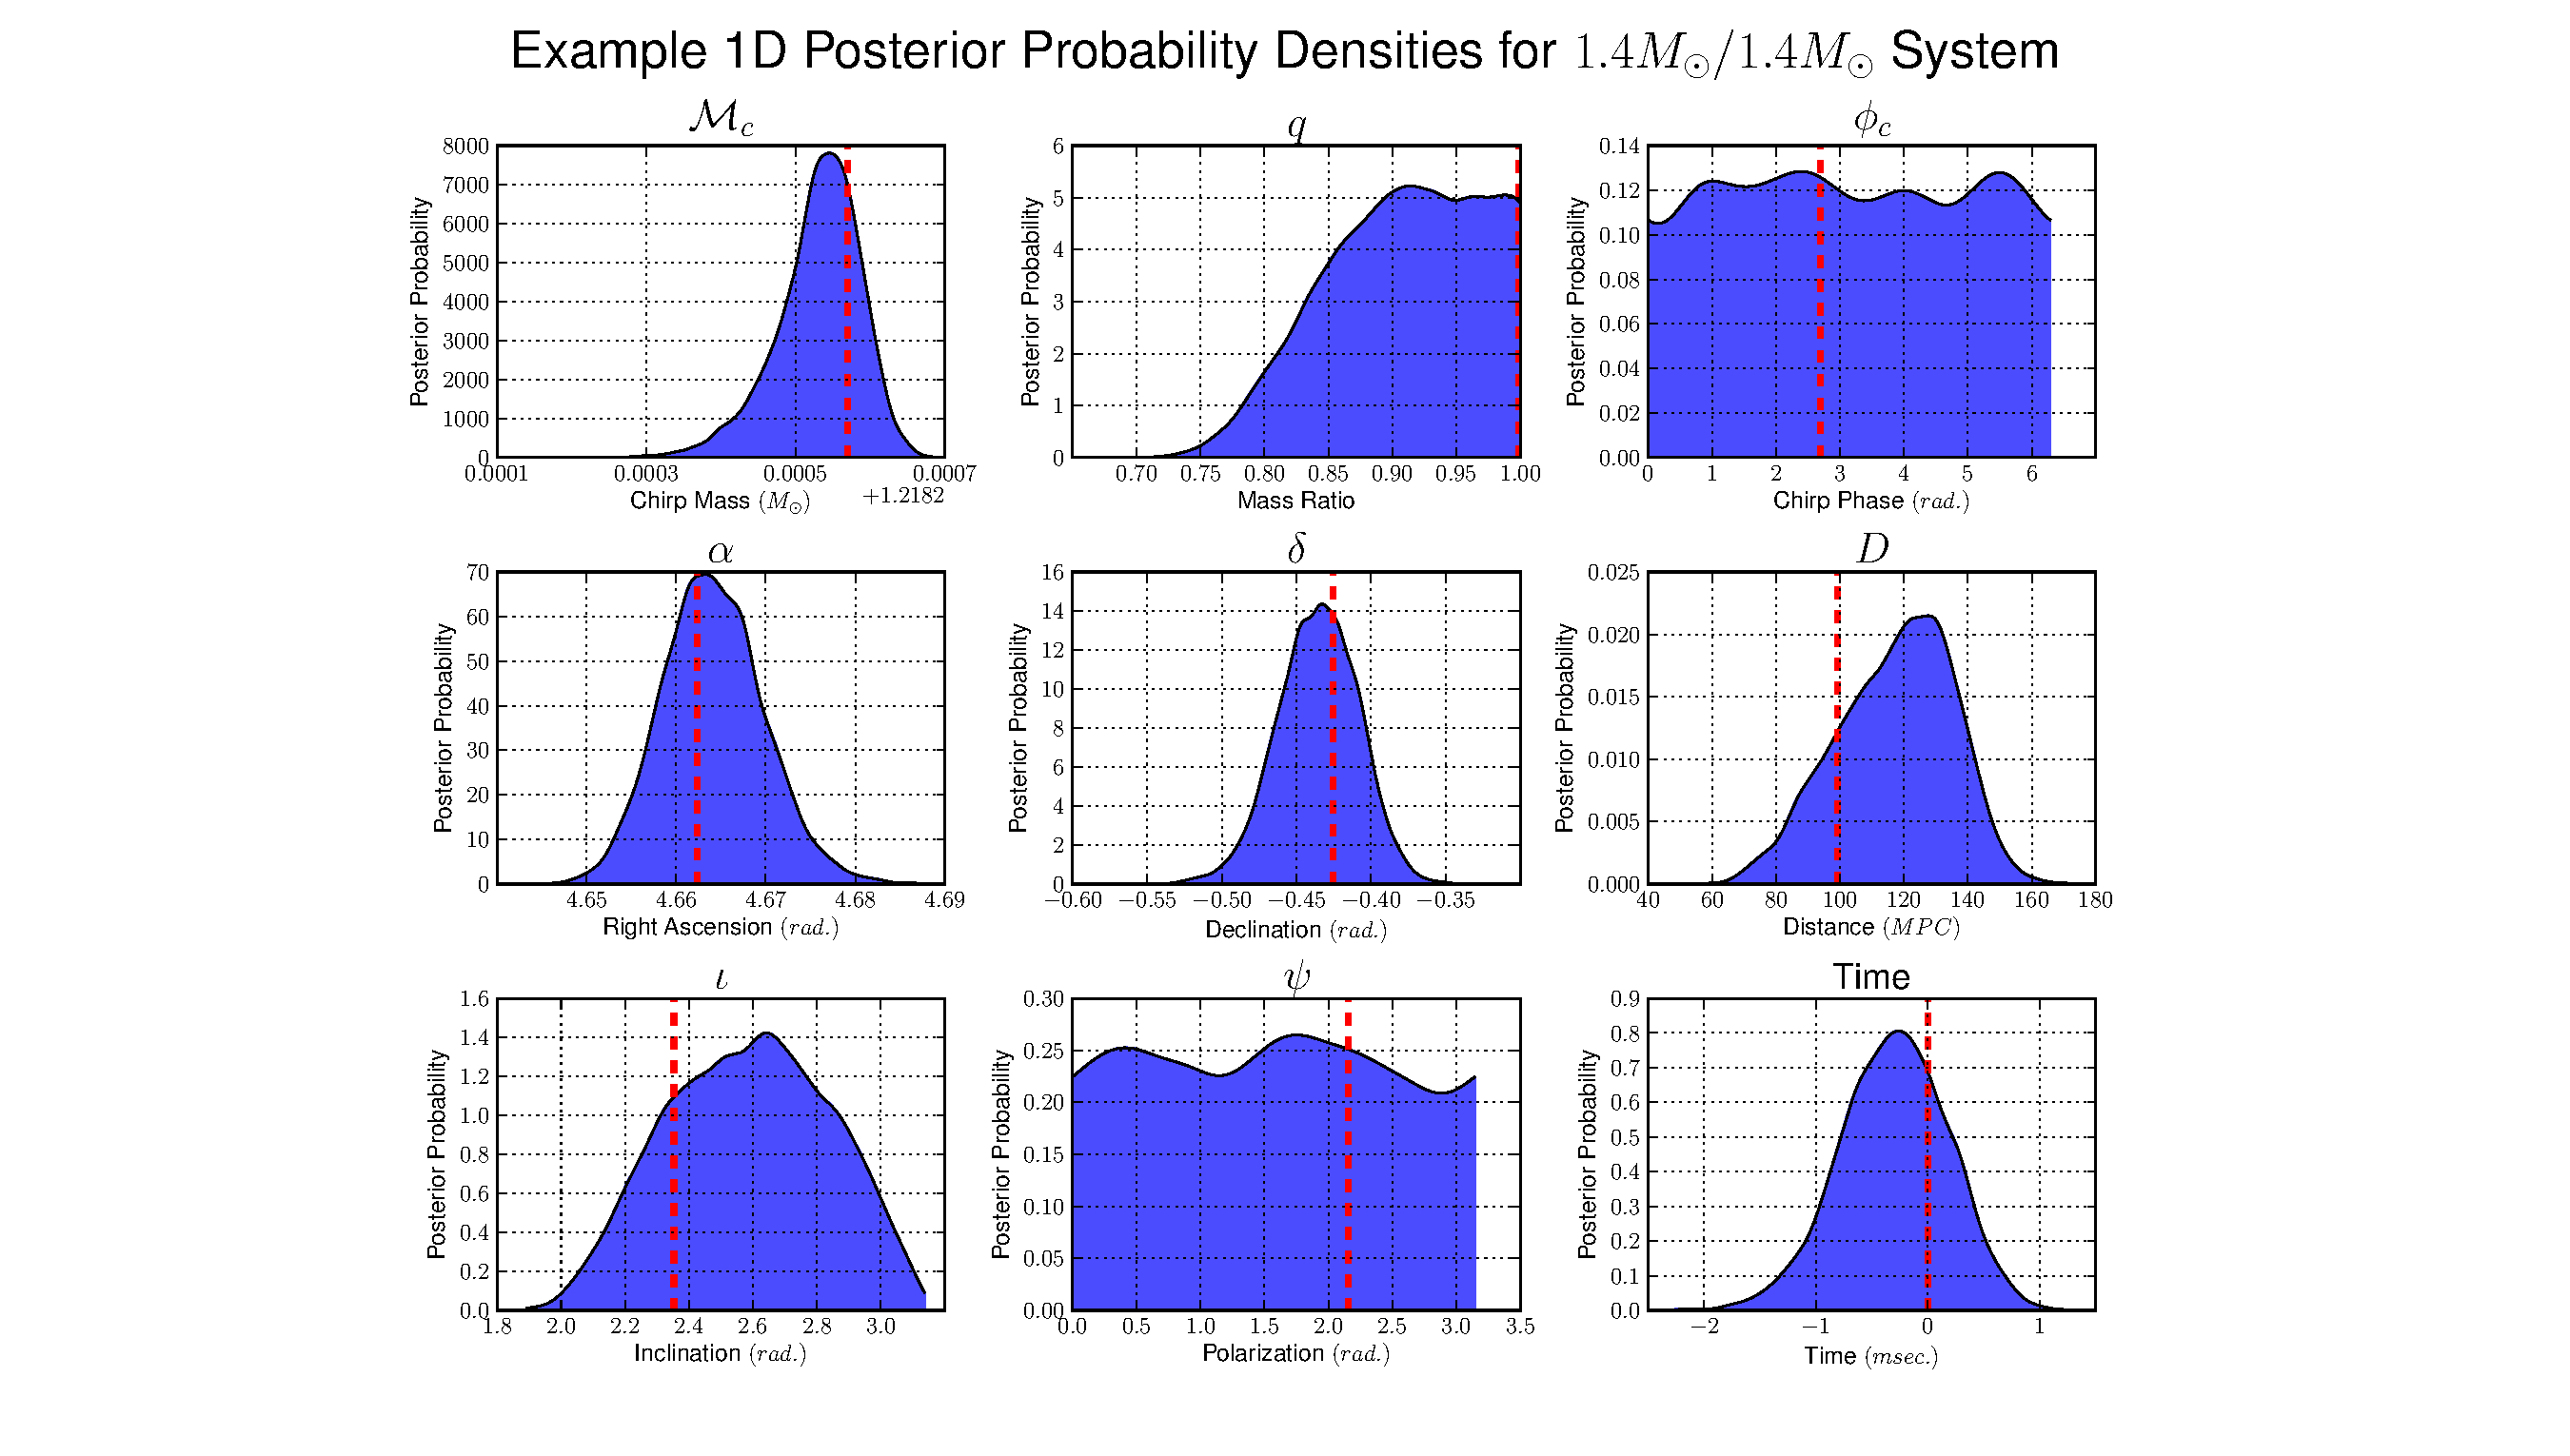
\includegraphics[trim=7cm 0cm 0cm 0cm, clip=true,scale=0.55]{9dpdf.pdf}
%\begin{array}{ccc} 
%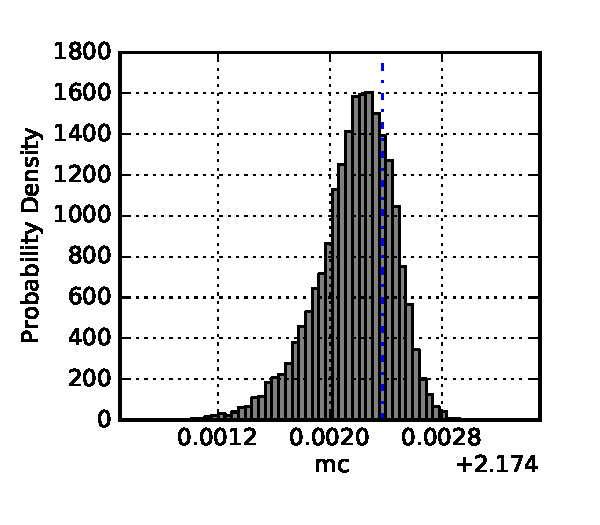
\includegraphics[width=2.2in]{1dpdfs/mc.pdf} &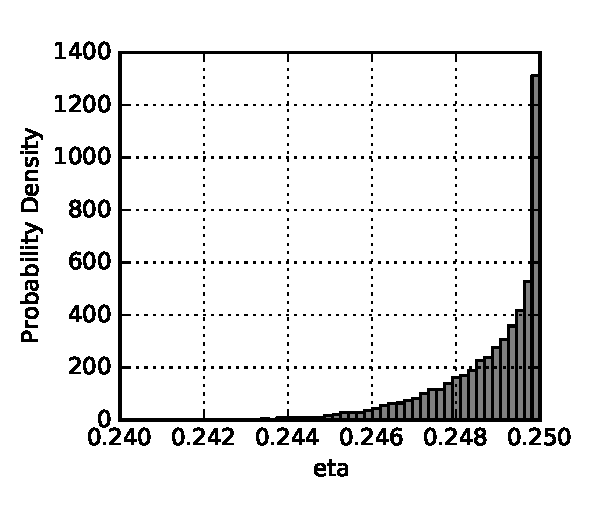
\includegraphics[width=2.2in]{1dpdfs/eta.pdf}  & 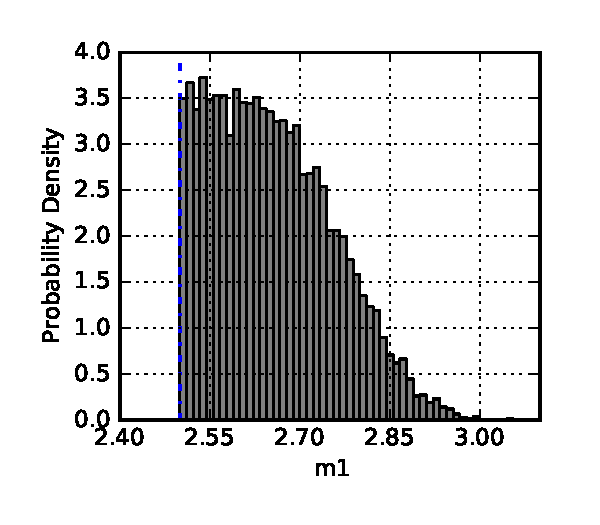
\includegraphics[width=2.2in]{1dpdfs/m1.pdf}\\
%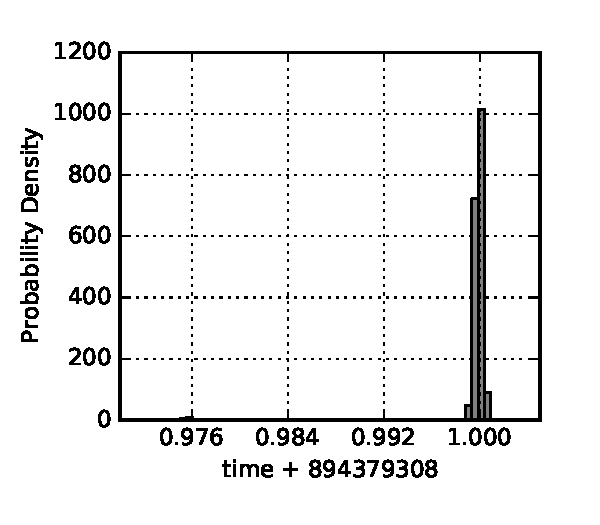
\includegraphics[width=2.2in]{1dpdfs/time.pdf} &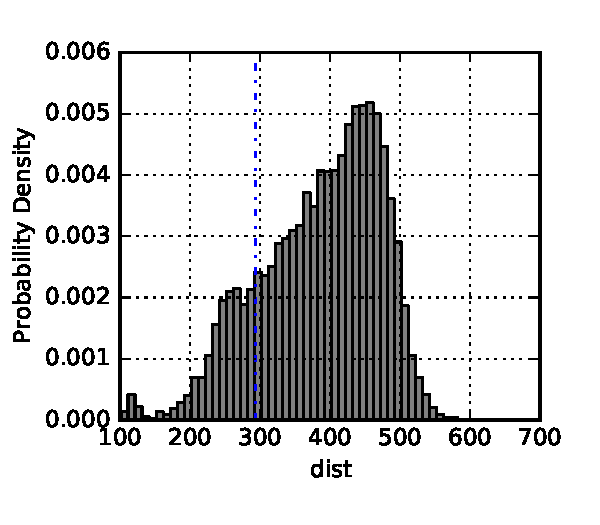
\includegraphics[width=2.2in]{1dpdfs/dist.pdf}  &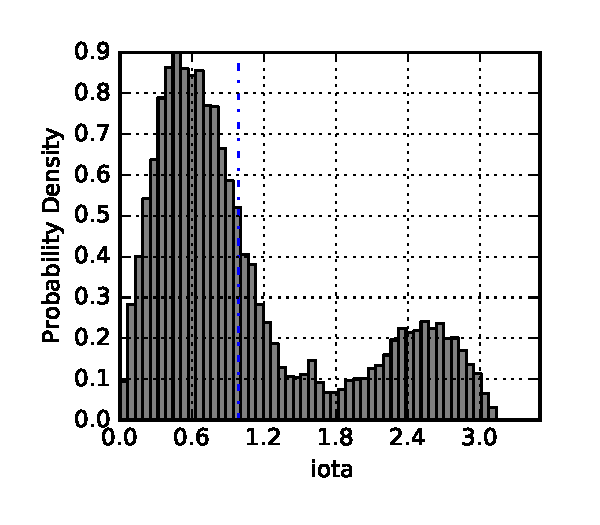
\includegraphics[width=2.2in]{1dpdfs/iota.pdf}\\
%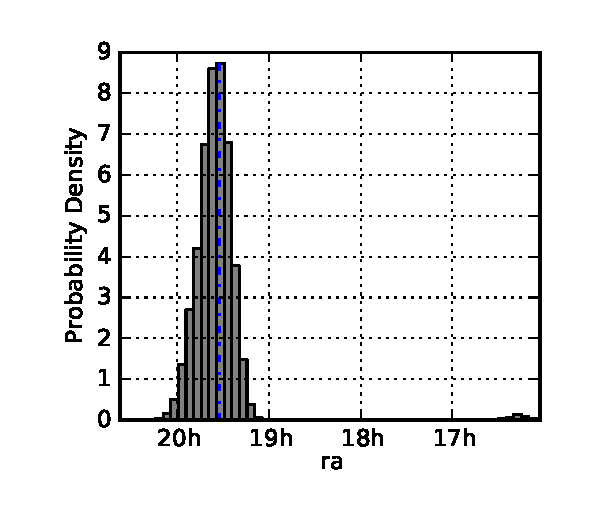
\includegraphics[width=2.2in]{1dpdfs/ra.pdf} & 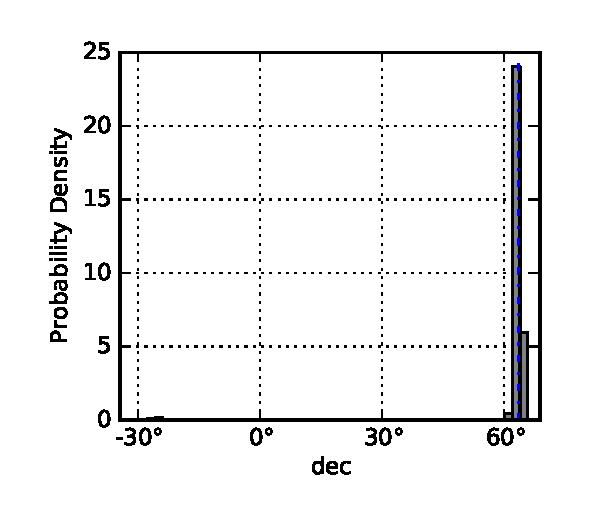
\includegraphics[width=2.2in]{1dpdfs/dec.pdf} & 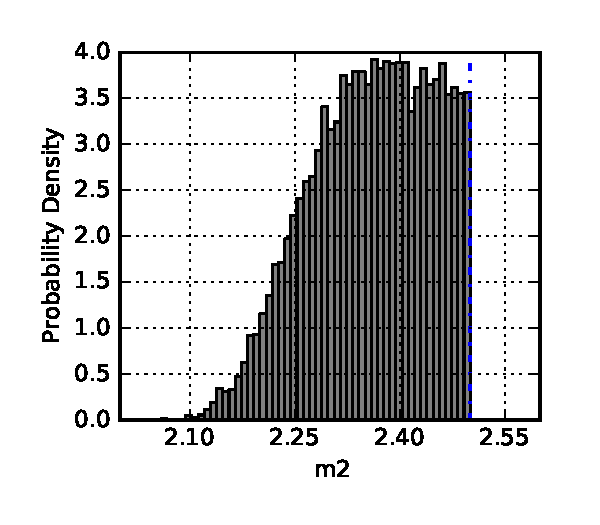
\includegraphics[width=2.2in]{1dpdfs/m2.pdf}
%\end{array}$
\caption{Marginalized 1D posterior probability density functions taken from a typical 
$1.4M_{\odot}/1.4M_{\odot}$ BNS system.  We have plotted each of the 9 parameters for 
our non-spinning BNS problem as stated in section \ref{waveformSection}.  Note how, 
even for parameters with excellent recovery, the peak of the 1D Gaussian is displaced from 
the injected value (in dashed red).  This is not due to a systematic bias, but is caused by the 
marginalization of a single dimension from the full 9D posterior space.  To better see this effect, 
compare the 1D PDF for $\mathcal{M}_{c}$ and $q$ with the 2D marginalized PDF in Figure~\label{9dPDF}}
\end{figure*}

Of the nine parameters in the domain of the waveform, only six are particularly physically
interesting: the masses of the two binaries, $M_1$ and $M_2$, the orbital inclination,
$\iota$, the angular position on the sky, $\alpha$ and $\delta$, and the luminosity 
distance of the source, $D$.  While the coalescence phase $\phi_c$, the coalescence time
$t_c$, and the wave polarization $\psi$ must be included in any parameter estimation of the 
waveform, they do not encode any information of particular astrophysical interest.
\footnote{For systems whose components are non-spinning.  The presence of intrinsic angular 
momentum will, in general, couple to the coalescence phase and wave polarization.}   

In Figure~\ref{9dPDF}, we provide an example of the nine, 1-dimensional marginalized posterior 
probability density functions recovered from a single $1.4M_{\odot}/1.4M_{\odot}$ BNS system. 
 These PDFs are the typical of the type of results that will be produced by parameter estimation
  studies in the advanced  detector era.  Notice that the peak of several parameters, including the 
  chirp mass, $\chmass$,  appears to be displaced from the true values in red.  This effect is due to 
  the reduction of the  9-dimensional PDF to a series of marginalized 1-dimensional PDFs. 
   For instance, the 1-dimensional PDF for chirp mass is marginalized via

\begin{equation}
p(\chmass | s) = \int _{\thpara \setminus \chmass} p(\thpara | s)~d(\thpara \setminus \chmass)
\label{mcMarginalization}
\end{equation}

\noindent where the notation $\thpara \setminus \chmass$ implies all
parameter of \eqref{parameterspace} except $\chmass$.  Other parameter and higher-dimensional marginalizations follow
 a similar convention.  In practice, the MCMC samples make this integral trivial: since the samples are distributed according 
to the posterior, \eqref{mcMarginalization} can be calculated by simply reading off the relevant samples in a single parameter, 
implicitly calculating a Monte-Carlo integral over all other parameters.



\subsection{Mass Parameters}
\label{massSection}


\begin{figure}[h!]
  \centering
 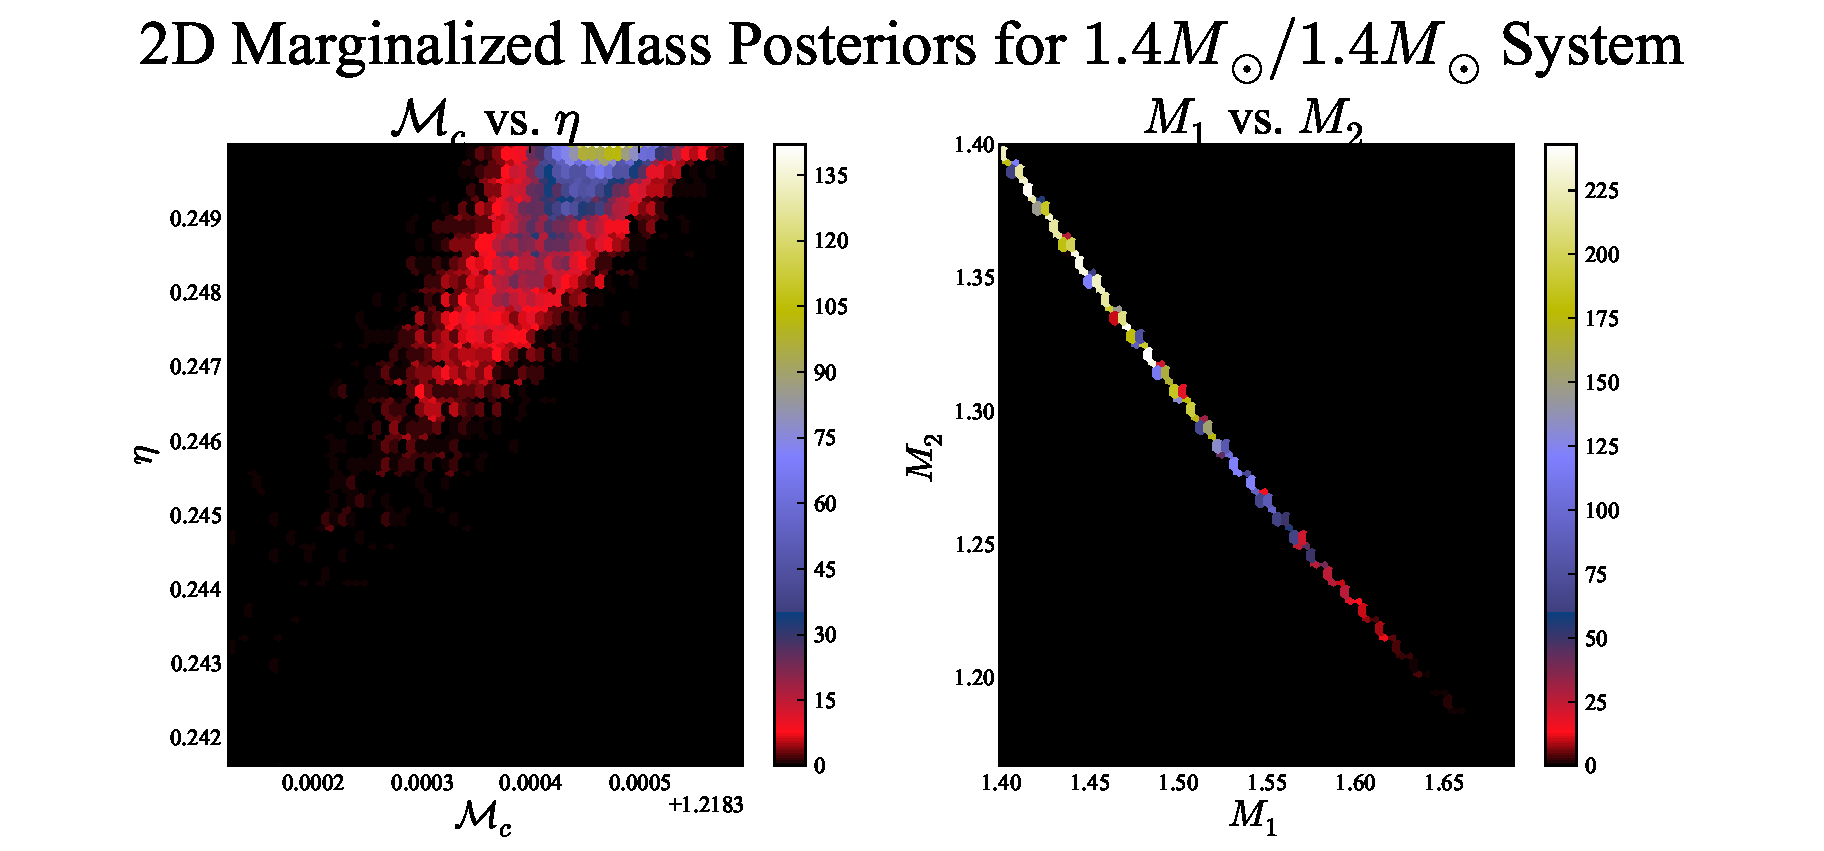
\includegraphics[trim=1cm 0cm 2cm 0cm, clip=false,scale=0.63]{1414masses2D.pdf}
 \caption{2D marginalized posterior probability density functions for the mass parameters recovered in typical a $1.4M_{\odot}/1.4M_{\odot}$ system.  The posteriors are plotted in terms of parameters used in the waveform, chirp mass ($\mathcal{M}_C$) and the mass ratio ($q$), and in the individual component masses of the binary ($M_1$ and $M_2$).  In the $\chmass$-$q$ space, the posterior would resemble a Gaussian if not for the limitation of $q \leq 1$.  The presence of the $q$ cutoff and the convention that $M_1 \geq M_2$ inform the non-Gaussian features present.  When projected as 1D marginalized posteriors, the component masses resemble the posterior PDFs shown in figure \ref{metaMassPDFs}.}
  \label{1414masses}
\end{figure}


\begin{figure}[h!]
  \centering
 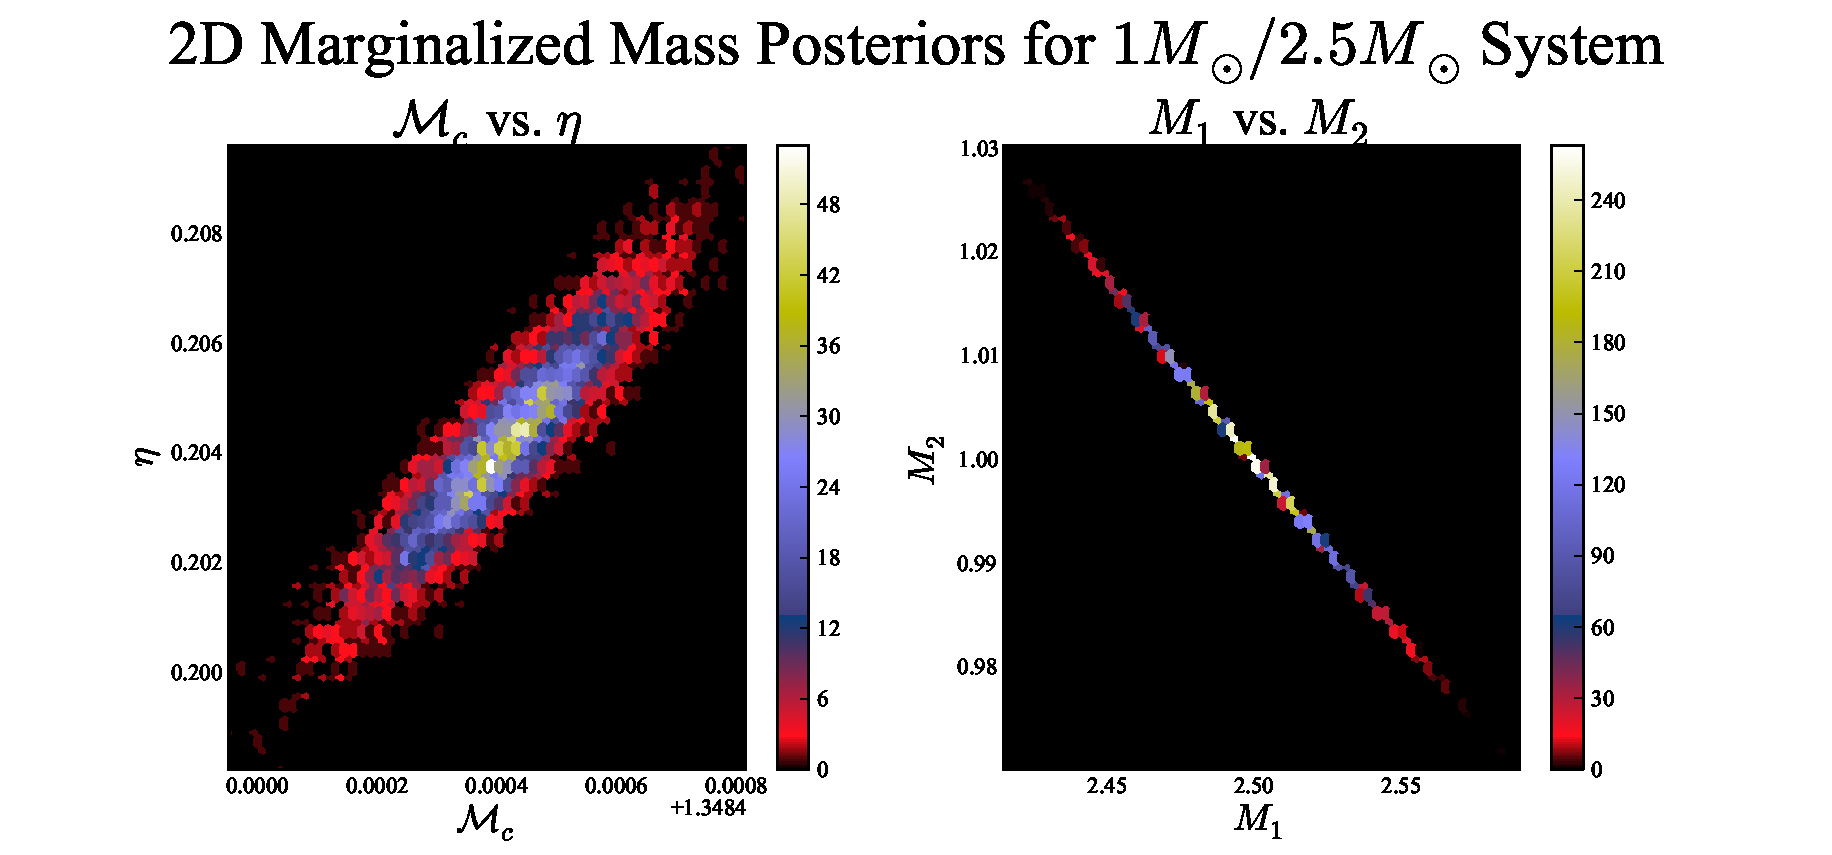
\includegraphics[trim=1cm 0cm 2cm 0cm, clip=false,scale=0.63]{125masses2D.pdf}
 \caption{Similar to Figure~\ref{1414masses}, for a typical $1M_{\odot}/2.5M_{\odot}$ system.  The unequal mass ratio displaces the posterior PDFs from the $q \leq 1$ present in the equal mass case, yielding a Gaussian PDF in both the $\chmass$-$q$ and $M_1$-$M_2$ spaces.}
  \label{125masses}
\end{figure}

\begin{figure*}[ht!]
  \centering
 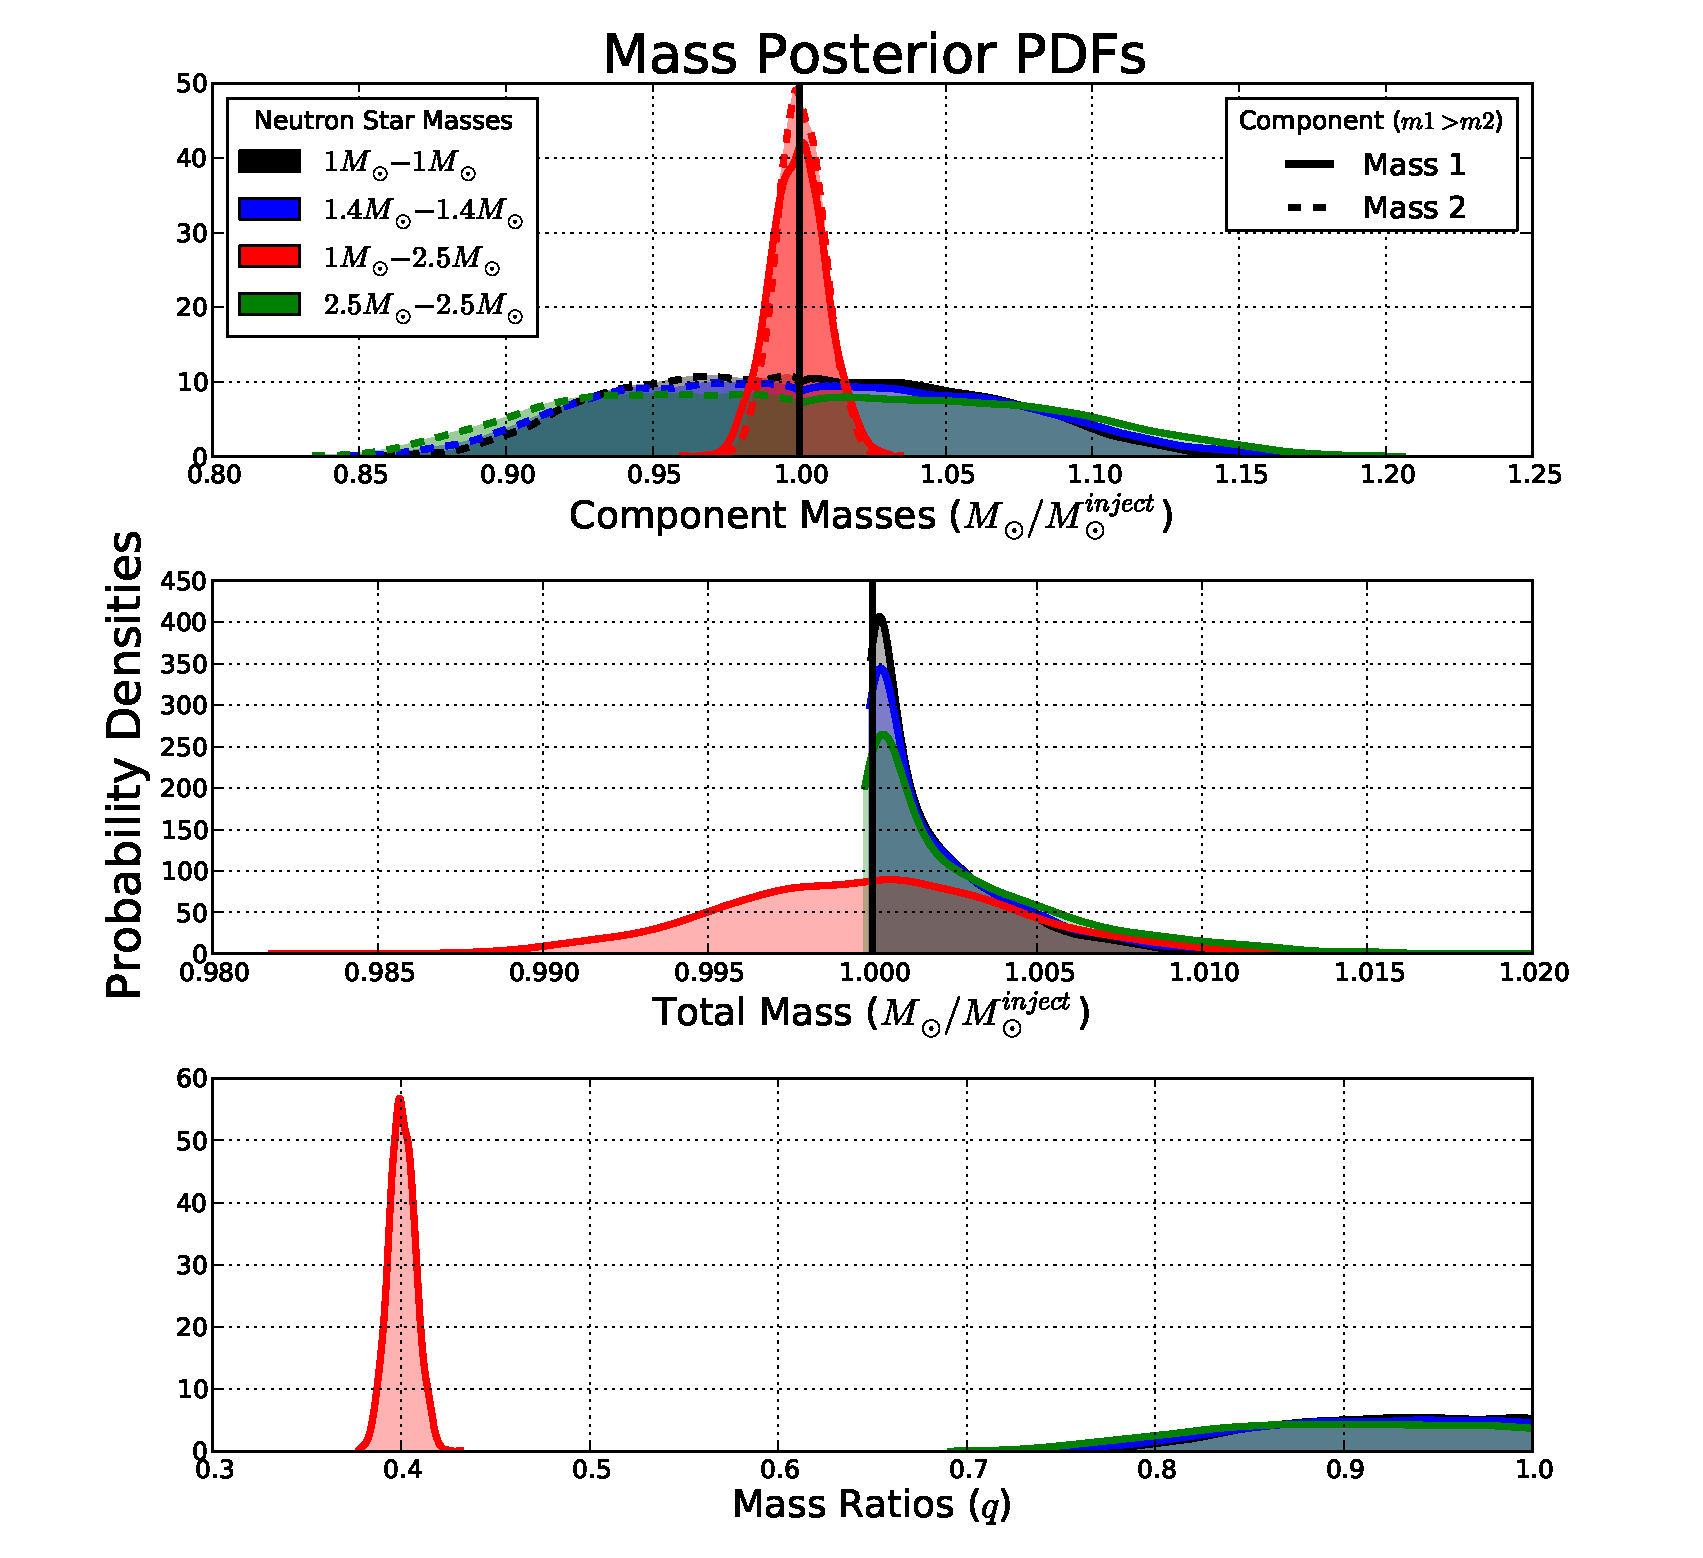
\includegraphics[trim=2cm 0cm 2cm 0cm, clip=false,scale=0.7]{newMasses.pdf}
 \caption{Mass PDFs for the four BNS systems, averaged over each of the 40 injections.  The average is reported since, in practice, there was quantitatively no difference between the recovered PDFs for different systems with identical masses and SNRs.  Systems with identical mass ratios but different total masses have quantitatively identical PDFs when normalized to the true total mass.}
  \label{metaMassPDFs}
\end{figure*}

Of the nine variables in our parameter space \eqref{parameterspace}, the two of immediate physical
interest are the two parameters, $\chmass$ and $q$, or correspondingly the direct masses 
of the two companions, $M_1$ and $M_2$.    As stated above, the ability of
Advanced LIGO/Virgo to construct a population of BNS masses will be one of the more useful applications
of gravitational-wave astronomy.

We find that there is virtually no difference between the mass PDFs of our different injected signals
within each mass bin.  While this may initially seem disconcerting, it is to be expected.  Recall that all of the BNS signals were injected with a network SNR of 20 into a zero-noise detector realization.  Furthermore, note that the mass parameters are the only two which directly effect the phase of the TaylorF2 waveform \eqref{phase}.  Therefore, as long as the injected mass parameters are identical within each mass system, and as long as the injected SNR is identical, the amount of recoverable information in each mass parameter should be almost identical, and for a sufficiently converged MCMC chain, the recovered posterior PDF should be identical.  

This effect can be summarized as follows: for non-spinning systems, the posterior probability of the masses,
$p(\chmass, q | s)$, does not depend strongly on the recovery of the extrinsic parameters, $\phi_0$ or $t_c$.  Therefore, 
systems with identical masses will produce identical mass PDFs.  The only noticeable difference will come from
 the specific realization of noise produced by the detector, which we address in Section \ref{noiseSection}.


%The ``almost'' in the previous sentence is to draw attention to one critical, neglected fact: while the mass parameters are independent of the injected signals position with respect to the detector network, the other parameters are certainly not.  Obviously many of the other parameters (i.e. sky location, polarization, distance, inclination, and time-of-arrival) all depend on the orientation of the binary with respect to each of the individual detectors.  Since our 9-dimensional parameter space can be highly correlated, it is entirely reasonable to assume that cross-correlations between the extrinsic parameters and the mass parameters will cause variation in the recovery of the individual injection PDFs.  

%In practice, it was found that the cross-correlations between the extrinsic parameters and signal time-of-arrival were several orders of magnitude \carl{[QUANTIFY]} below the uncertainties in $\chmass$ and $q$.  It should be noted that, in practice, this will \emph{not} be the case: in reality, the noise power-spectral density of each detector varies as a function of time, including both natural variations in sensitivity and detector glitches \carl{[CITE]}.  In such a case, the base sensitivity of a gravitational-wave detector to even the easiest to recover parameters will vary as a function of position and time.  

In Figures~\ref{1414masses} and~\ref{125masses}, we show the marginalized 2D posterior PDFs of our
 mass parameters for  prototypical equal mass and unequal mass binaries.  We include the PDF in both
  the $\chmass$-$q$ space (relevant for the waveform and the MCMC algorithm), and the more physically 
  interesting component mass space ($M_1$-$M_2$).  Although only the $1.4M_{\odot}/1.4M_{\odot}$ system
   is included in Figure \ref{1414masses}, the PDF is quantitatively identical to the other equal mass cases, 
   modulo a scaling factor. 

To condense the results into a single figure of merit, we average the 1-dimensional mass PDFs into a single 
posterior probability for the system.  See Figure~\ref{metaMassPDFs}.  Notice how when averaged and
 normalized to the injected values, the recovery of the component masses depends only on the mass ratio.  
 Furthermore, for systems with equal component masses, the posterior barely extends beyond 15\% of the injected values.  
 If one assumes that the threshold between black
   holes and neutron stars lies at approximately $3M_{\odot}$, then it might be assumed that
   the mass recovery would allow one to discriminate between black holes and neutron stars.
   
Unfortunately, this will not be feasible in practice.  We have neglected the spin of the binaries, which will be highly
correlated to the masses.  This coupling means that a higher-massed spinning black hole systems can produce
 waveforms very similar to non-spinning, low-mass systems, making it extremely difficult to discern between non-spinning 
 neutron stars
 and spinning, more massive black holes \citep{Baird2013,Hannam2013}.  However, the situation is not hopeless: if the spins are misaligned, the spin 
 vectors will couple to the orientation of the binary (encoded in the three angles $\phi_0$, $\iota$, and $\psi$) via
 relativistic precession.  It remains to be seen if using fully spinning waveforms will make it possible for Advanced\
  LIGO/Virgo to discern binary neutron stars from their spinning black hole counterparts. 

In Table \ref{ciTableIntrinsic}, we list the 65\% fractional credible intervals for the mass parameters.  We find that the 
component masses for equal mass systems can be isolated to between 6\% and 9\% fractional uncertainty at the 65\% credible interval.  This value drops to less than 2\% for the components of the unequal mass systems.  Again, this 
neglects the effects of spin which can substantially increase these values.


\subsection{Inclination and Distance}
\label{idSection}

   
\begin{figure}[h!]
  \centering
 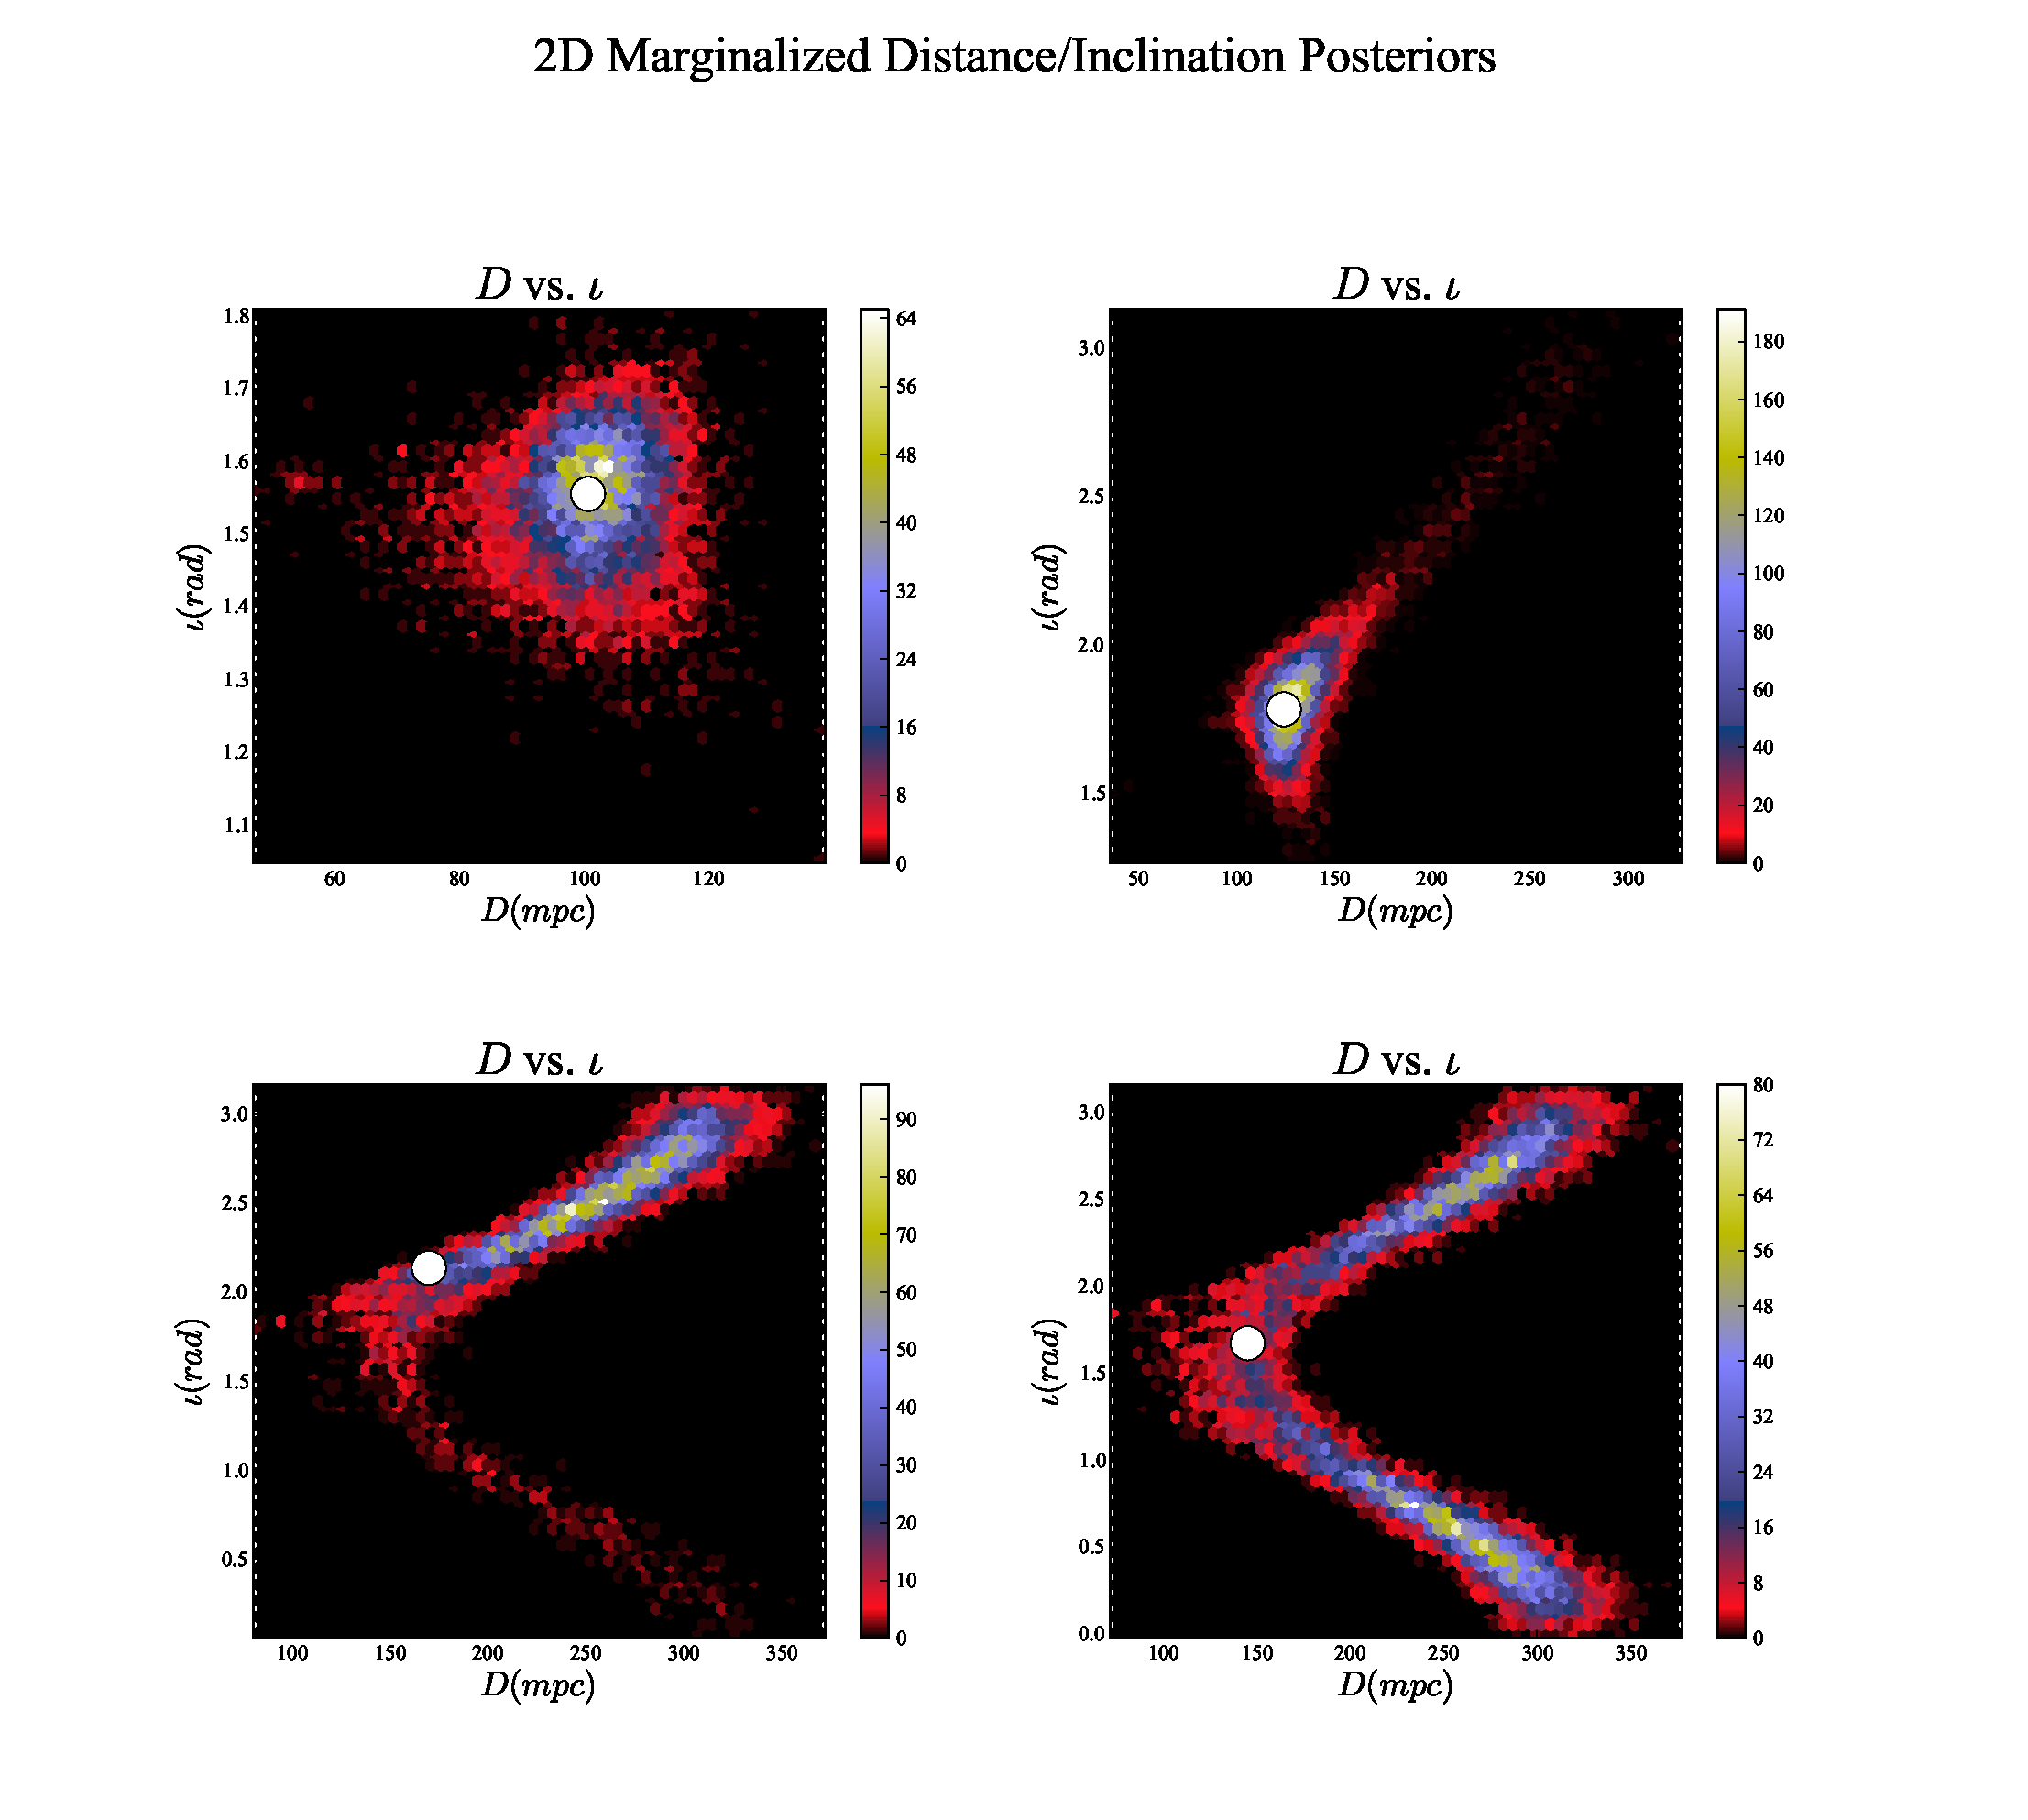
\includegraphics[trim=0cm 0cm 0cm 0cm, clip=true,scale=0.75]{distIota2D.pdf}
 \caption{Typical marginalized 2D mass PDFs for luminosity distance $D$ and orbital inclination $\iota$. Notice the bimodal 
 distribution on the first PDF, that can occur when a system is detected nearly ``edge-on'' ($\iota \approx \pi/2$).  In general,
 the degeneracy between distance and inclination forces the PDF into one of these two paths when the system is not edge-on,
  as seen in the second and third PDFs.}
 \label{distIotaPDF}
\end{figure}

Binary neutron star systems (along with neutron star/black hole systems) are one of the best candidates for progenitors of short-hard gamma-ray bursts \citep[and references therein]{Nakar2007}.  After merger, the remnant is believed to emit the burst along the axis of orbital angular momentum, making the inclination of the binary system of particular interest to gamma-ray astronomy \citep{LSCGRB2010,Corsi2012}.  The inclination is detected as a relative amplitude difference between the two gravitational-wave polarizations, such that to lowest order

\begin{align}
h_+(f) &= \frac{1+\cos^2(\iota)}{2 D} \tilde{h}(f) \nonumber \\
h_\times(f) &= i \frac{\cos(\iota)}{D}\tilde{h}(f)
\end{align}

\noindent It should be apparent that the luminosity distance $D$ and the inclination $\iota$ can be highly correlated in any parameter estimation study.

Given this degeneracy, it should come as no surprise that the 2D marginalized posteriors of distance
 and inclination are the broadest of the six physically interesting parameters.  Four typical 2D PDFs are
  presented in Figure~\ref{distIotaPDF}.  Notice the bimodal uncertainty 
present in the top 2D PDF along the $\iota$ axis, due to the similarity between the evaluated
 likelihoods at $\iota$ and $\iota + \pi/2$.  As the majority of the information extracted via parameter 
 estimation is from the phase of the signal, the recovery of a posterior in $D$-$\iota$ space will be 
 limited, even during the Advanced LIGO/Virgo era; however, there if a gravitational-wave signal is 
 matched to a detected SGRB counterpart (which may occur at the rate of $\sim 3 yr^{-1}$ in Advanced LIGO/Virgo, 
 according to \cite{Metzger2013}), the optical information about the orbital inclination
 will provide an additional constraint on the D-$\iota$ space, vastly improving the luminosity distance recovery
 quoted here.
 
 
In Table \ref{ciTableExtrinsic}, we list the averaged 65\% confidence intervals for distance and inclination.  
Notice that the uncertainties on distance can be extreme, from tens to hundreds of $mpc$.  When discussing
the inclination angle, we elected to use $|\cos(\iota)|$, as this maps the occasional bimodal structure into
a single PDF, 
 and observing a compact merger at $\iota$ and $\iota + \pi/2$ should yield identical physics.  
%Since $|\cos(\iota)|$ maps the bi-modal structure in the inclination PDFs seen in Figure \ref{distIotaPDF} to a single
%mode, the uncertainties in $\iota$ will sufficiently small \carl{[QUANTIFY]} to provide coincident information on
%GRB beaming angles.

\subsection{Sky Localization}
\label{skySection}
 
Unlike the mass parameters, the recovery of the position on the sky is highly dependent 
on the location of the source with respect to the detector network in question. 
For the HLV configuration, the three-detector network can only localize signals to one of
two points in the sky.  That is, when using only time-of-arrival information, there is 
equal support in the probability density functions near true location and near the 
point reflected through the plane formed by the three detectors.  See  \cite{Fairhurst2011} for
 a global analysis of time-of-arrival accuracy for various network configurations, including those considered
 here.  
  
  
  In practice, however, additional information from the wave polarization and the relative difference
  in SNR between individual detectors can break this plane-reflected degeneracy,
   leading to a bi-modal distribution with significantly more support in one mode of the PDF.
     By fitting for the sky location and the polarization simultaneously, the MCMC can often identify
   the correct mode on the sky.  For the four-detector configuration, this concern is irrelevant: even with time-of-arrival
   data alone, the HLVI network can constrain any source to a single mode on the sky.  Even then, there are still locations 
   on the sky in which two or more detectors are not sensitive to the gravitational-wave signal, distorted, non-Gaussian PDFs.  

The sky location uncertainties for HLV and HLVI are shown in Figures \ref{2525SkyLocHLV}
 and \ref{2525SkyLocHLVI} respectively.  We show all four mass bins together, since in practice
  the mass of the signals has no effect on the recovery of the sky location.  Only the location on 
  the sky, the network configuration, and the other extrinsic parameters were found to be relevant.  
  In particular, notice the increase in efficiency between the HLV configuration and the HLVI 
  configuration.  In the HLV configuration, there exist points on the sky in which the signal was injected
  near the plane of the detector network.  This causes the elongated, ``banana-shaped'' PDFs seen in
  Figure \ref{2525SkyLocHLV}.  In the HLVI configuration, the plane is no longer relevant, and there are substantially
  less regions in which only two detectors see a sufficiently strong signal.  
  See \cite{Veitch2012} for a more detailed comparison of the sky-localization benefits of the HLVI 
  configuration verses the three-detector network.  As previously, the quantitative results for the two network configurations
  are reported in Table \ref{ciTableExtrinsic}.



\begin{figure*}[ht!]
  \centering
 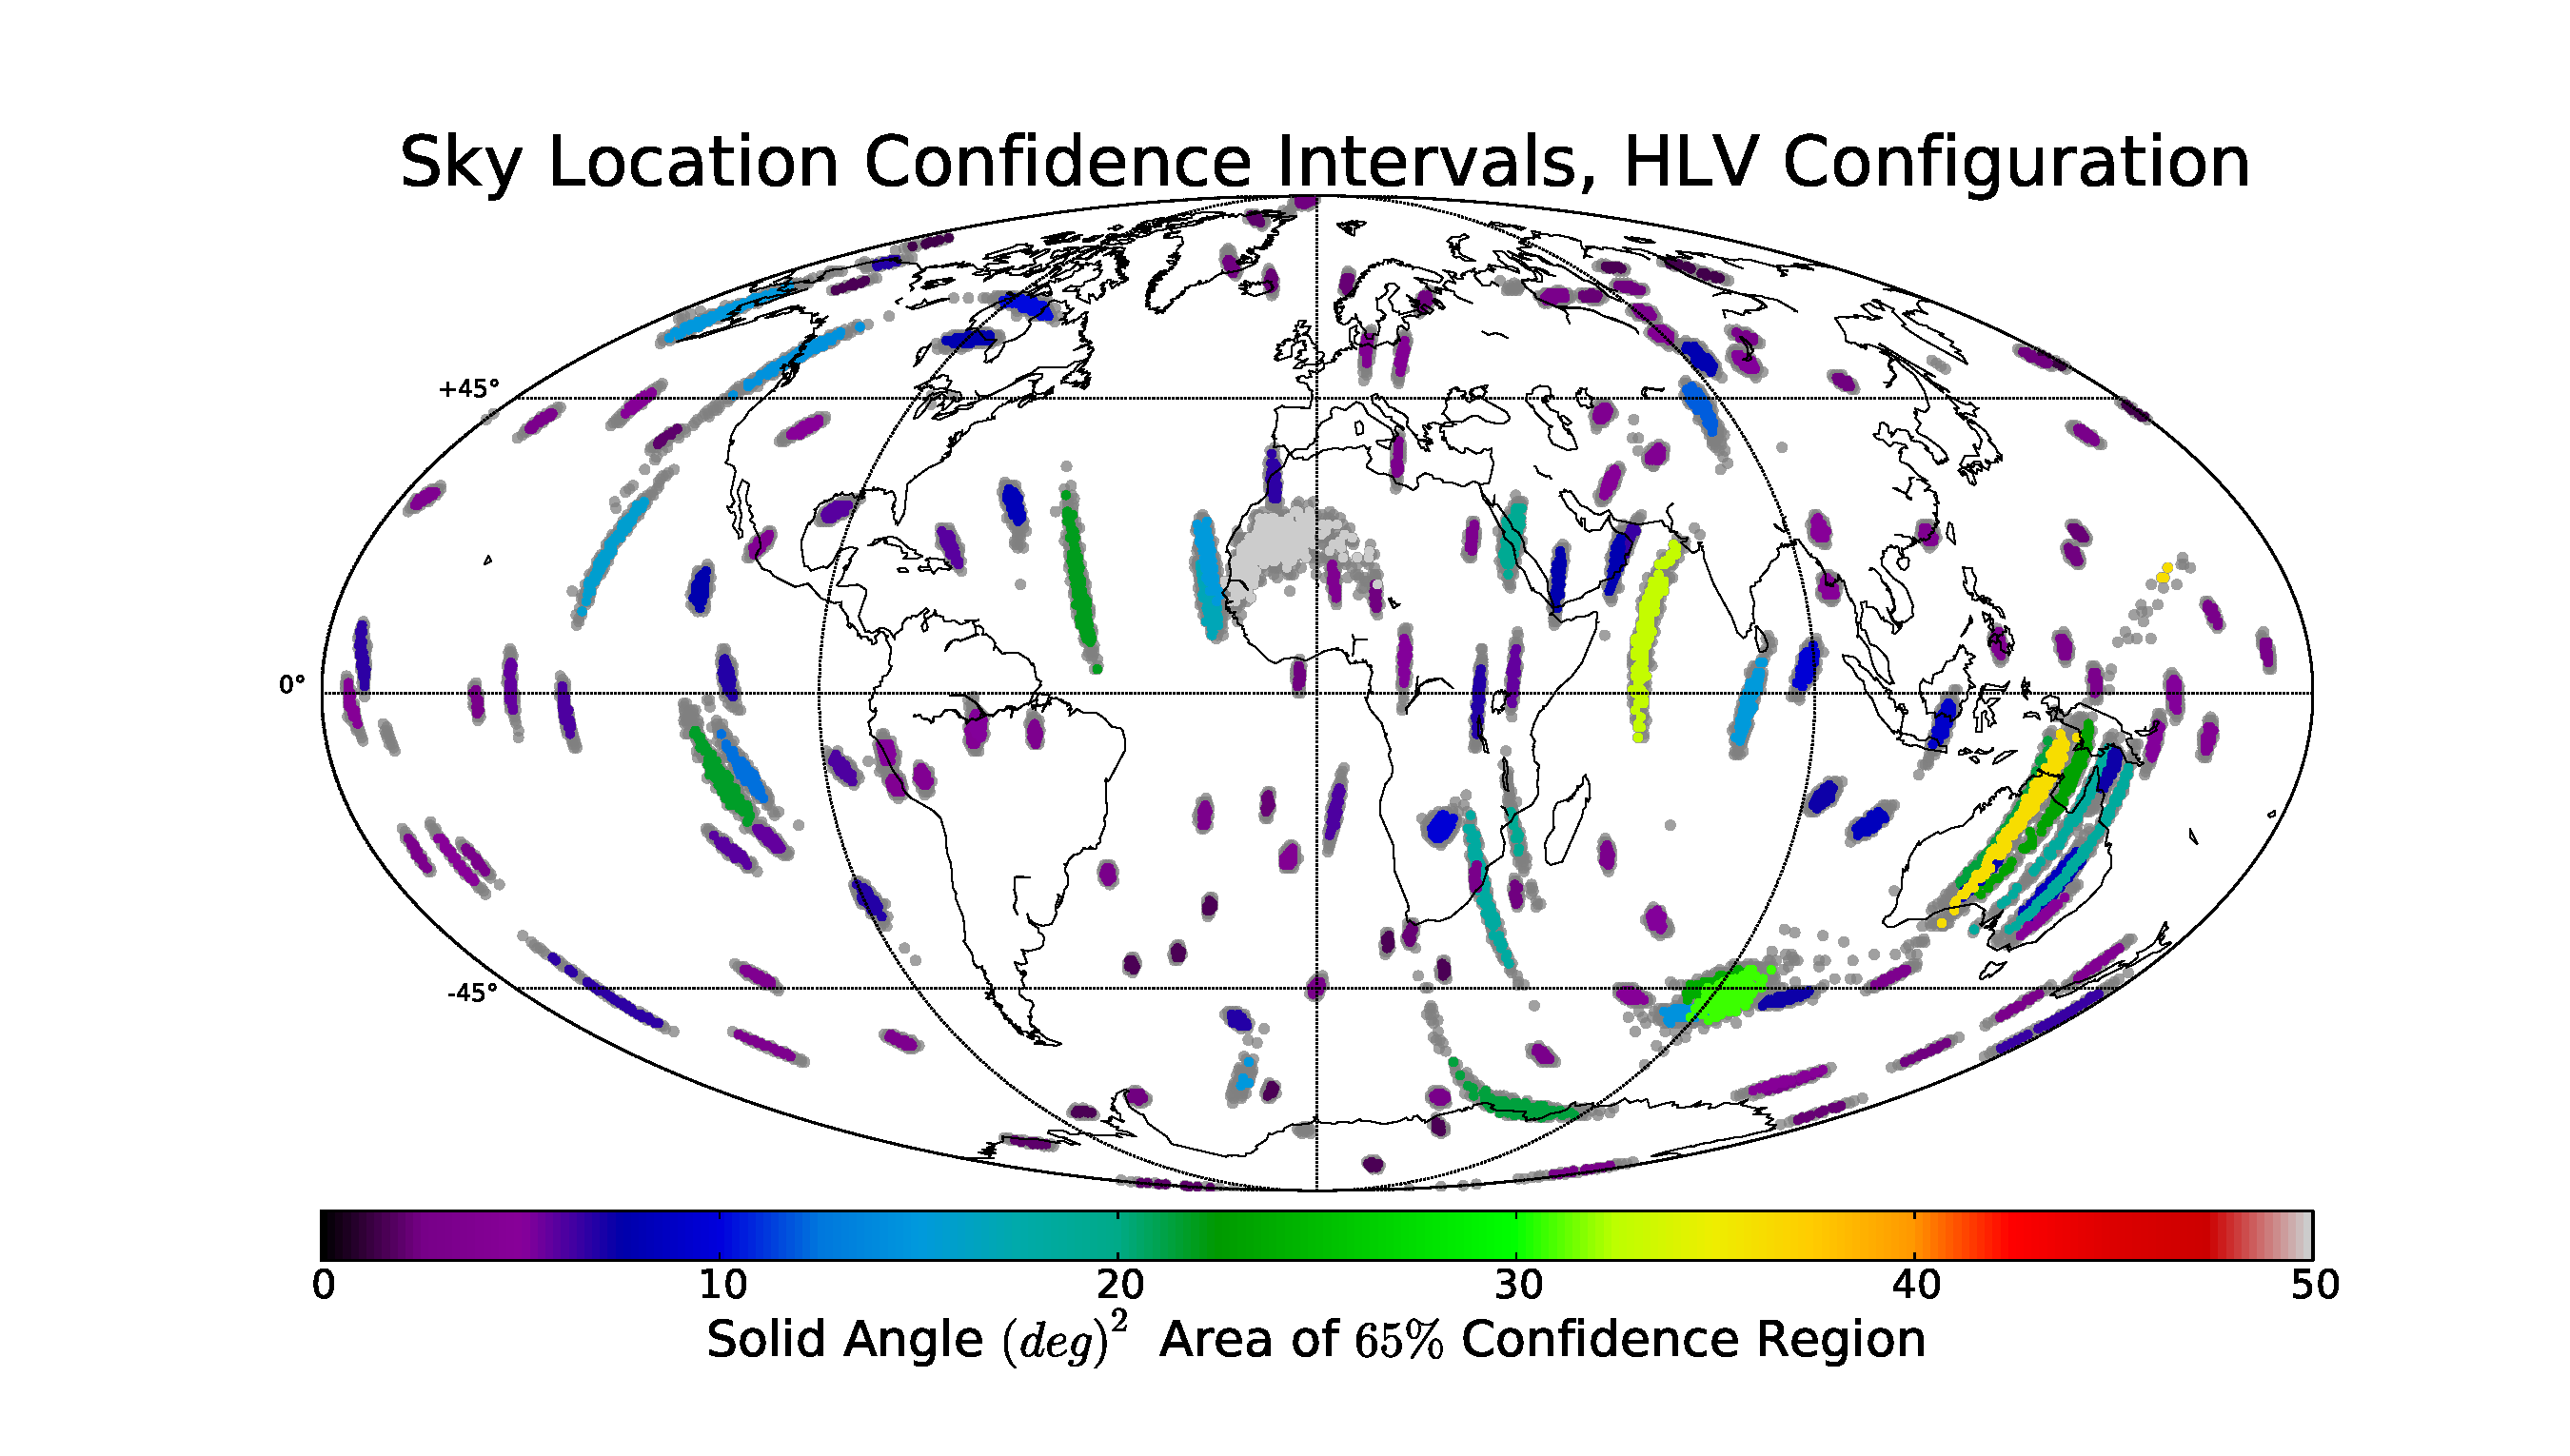
\includegraphics[angle=0,scale=0.4, trim=5cm 2cm 3cm 0cm]{HLVsky.pdf}
 \caption{The uncertainty on the sky of 160 BNS systems in the HLV detector configuration.  Each region represents a single injection, with the colored central region representing the 65\% uncertainty region on the sphere, and the gray region representing the 90\% uncertainty region.  The color scheme indicates the total solid angle size of the 65\% region.  Note the similar shape of the uncertainty regions at particular points; this is due to the specific realization of our network pattern sensitivity.}
 \label{2525SkyLocHLV}
\end{figure*}

\begin{figure*}[ht!]
  \centering
 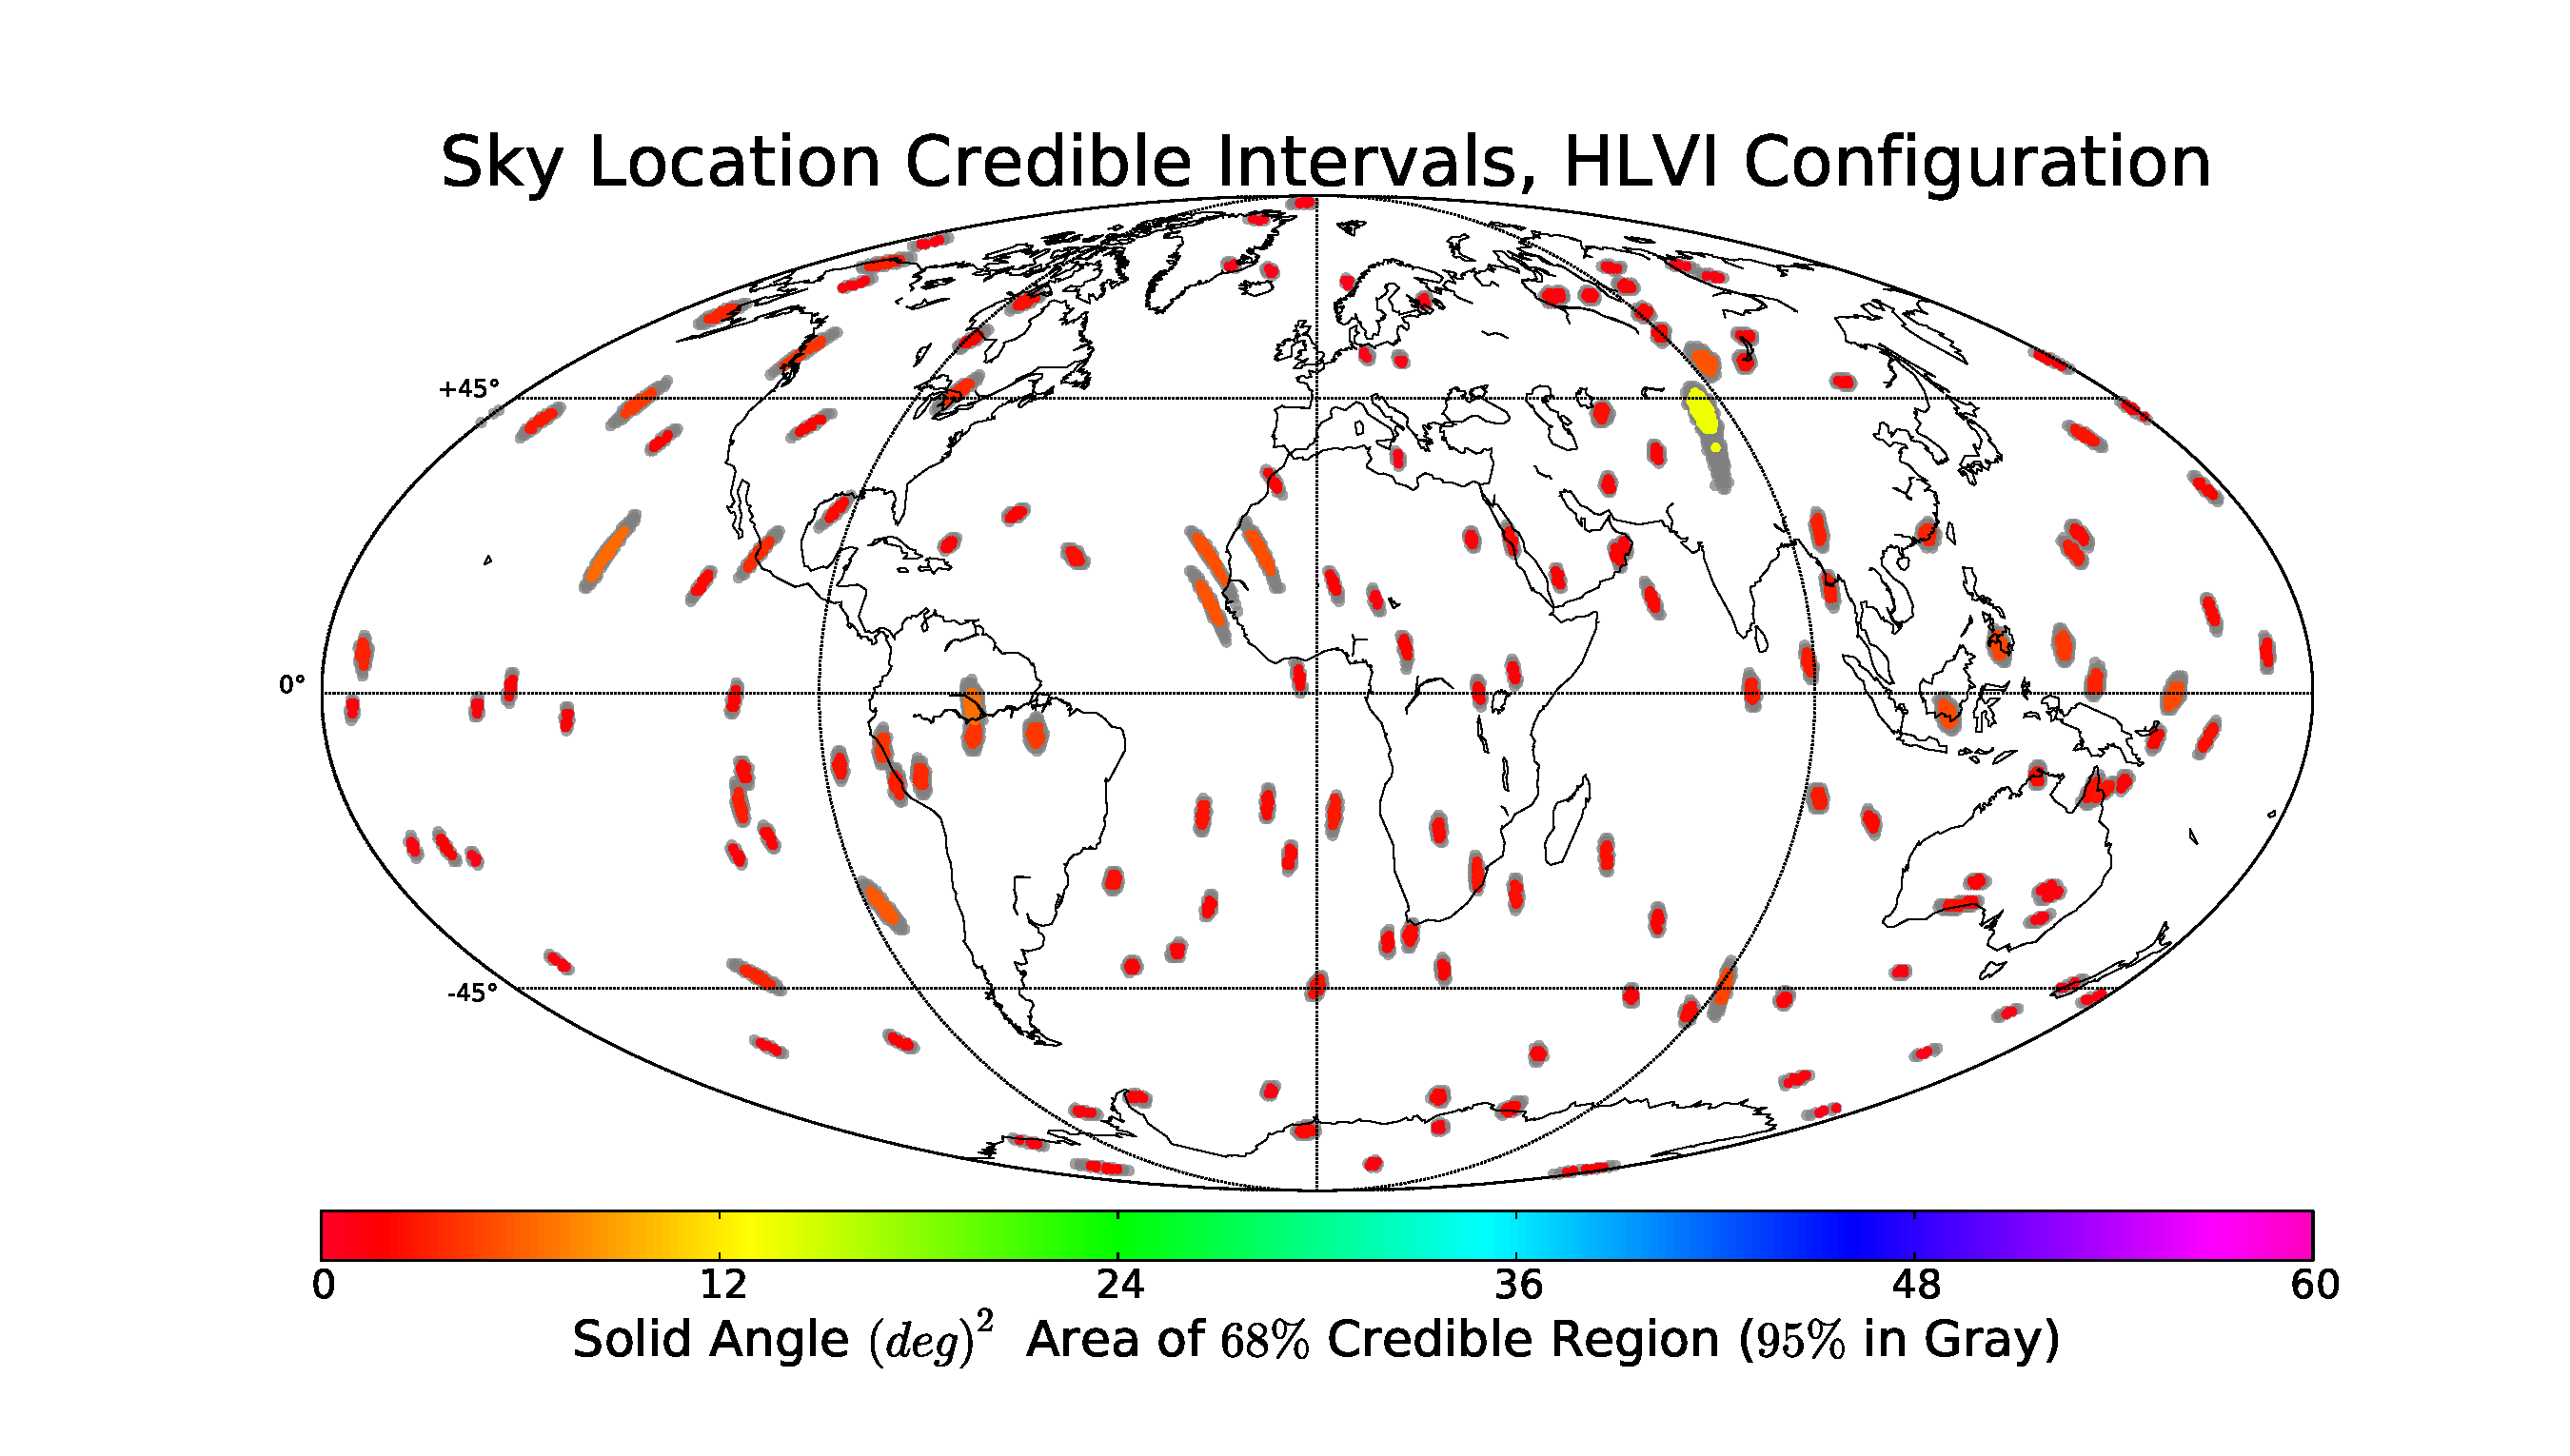
\includegraphics[angle=0,scale=0.4, trim=5cm 2cm 3cm 0cm]{HLVIsky.pdf}
 \caption{The same as Fig \ref{2525SkyLocHLV}, except for the HLVI detector configuration.  Note the substaintally lower average uncertainties on the skies for the majority of the injections.  Also note the lack of large, ``banana-shaped'' uncertainties that were recovered by the HLV configuration.  The two improvements are due to the breaking of the degeneracy in sky location recovery that is facilitated by the transition to a four-detector network.} 
 \label{2525SkyLocHLVI}
\end{figure*}
  

\subsection{Varied Noise Realizations}
\label{noiseSection}

\begin{figure}[ht!]
  \centering
 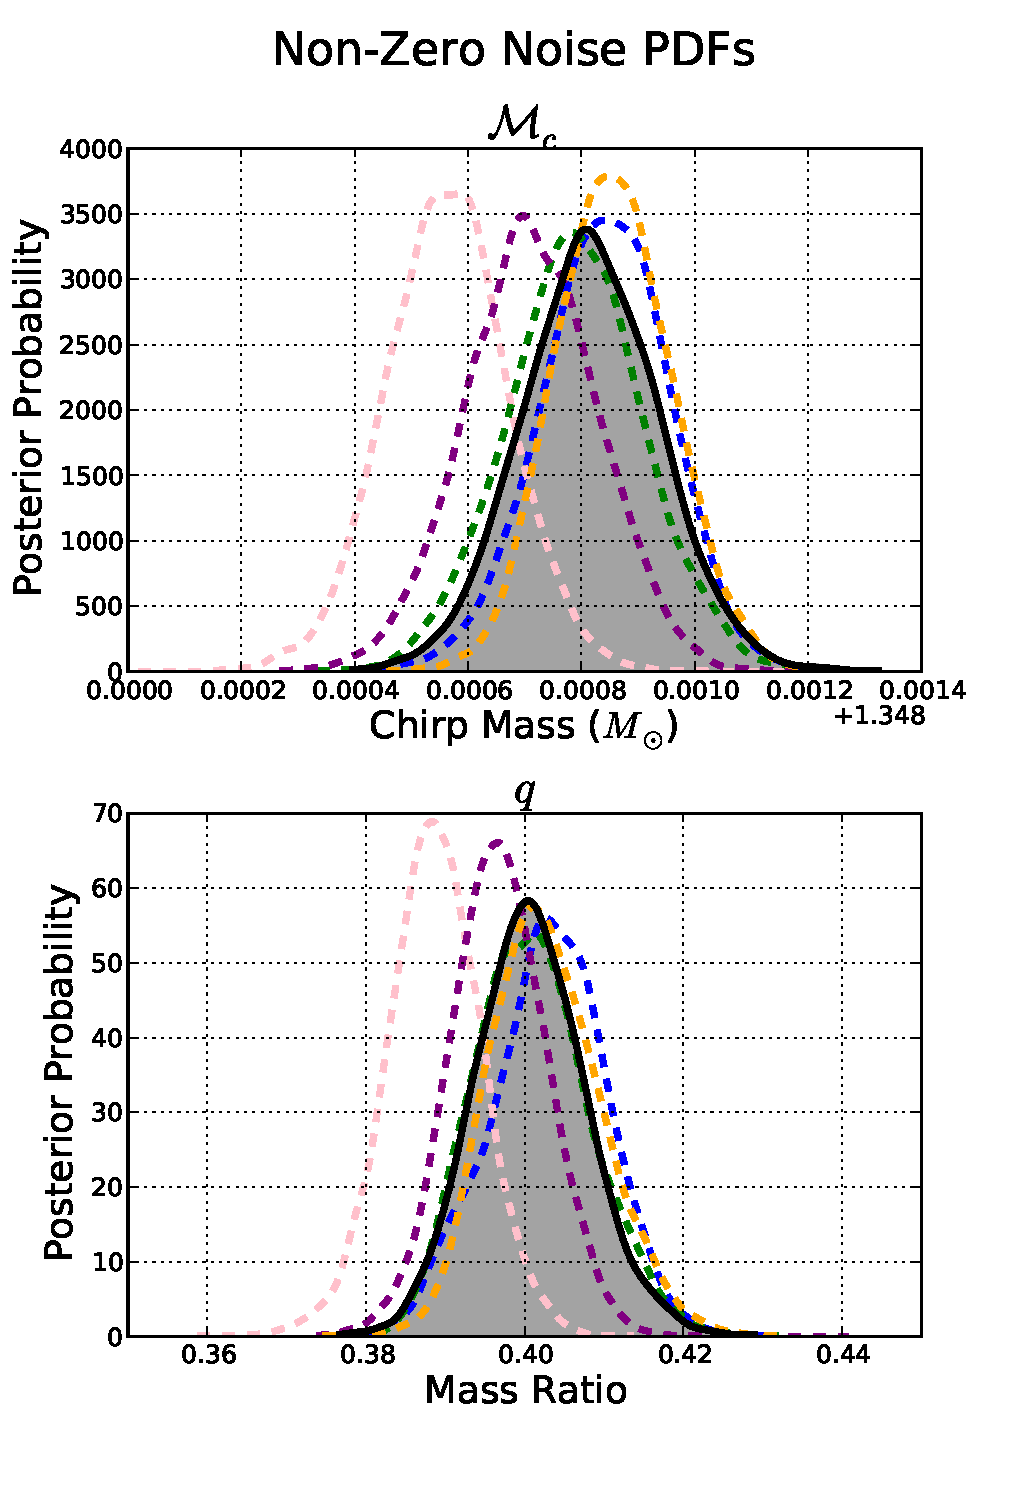
\includegraphics[trim=0cm 0cm 0cm 0cm, clip=true,scale=0.52]{noisePDF.pdf}
 \caption{The effects of a non-zero noise realization on the recovered PDF for five different Gaussian realizations of the Advanced LIGO noise curve.  Each PDF represents the recovery of the same $1M_{\odot}/2.5M_{\odot}$ signal in a different noise curve, picked at random from the Gaussian colored noise defined by the Advanced LIGO power spectral density.  Notice how the curve is relatively unchanged, but usually assumes a Gaussian PDF displaced from the true value.  This only holds true for glitch-free data, which is an unrealistic idealization when compared to real data.}
 \label{noisePDFs}
\end{figure}
  
  

We have performed the current analysis on zero-noise injections for two reason.  First, the results of a zero-noise 
analysis are identical to those that would be achieved by averaging the results of multiple identical injections 
in different Gaussian noise realizations, as was argued in Section \ref{waveformSection}.  The second reason is simply
that no good model exists for the true (decidedly non-Gaussian) noise that will arrive with a single detection candidate,
Each detection will occur in noisy data, with a specific realization of the PSD provided and with 
possible instrumentation and environmental glitches.  In the case of a unique Gaussian realization
of the Advanced-LIGO noise curve, each realization causes the maximum likelihood of the posterior probability 
distribution to be translated away from the true value; however, these displacements are drawn
according to the zero-noise distribution \citep{Inadequacies}.  Once averaged, the mean
uncertainties should be equal to the uncertainty drawn from the zero-noise runs.  

As a demonstration of this, we injected a single $1M_{\odot}/2.5M_{\odot}$ system, 
detected in HLVI,  into 5 separate realizations of Gaussian noise colored by the Advanced LIGO PSD, 
and compared the results to the same MCMC recovery in the zero-noise case.  This example
can be seen for one-dimensional marginalization of $\chmass$ and $q$ in Fig. \ref{noisePDFs}.  In effect, the ``real answer'' that will be recovered is a single PDF with similar 
width to the zero-noise PDF, but with the peak likelihood displaced from the true value.  

Of course, the largest concern for gravitational-wave parameter estimation will not be the specific
realization of Gaussian noise, but the effects of glitches in the data.  These time-series 
glitches have a variety of well-known and not-so-well-known physical causes in the instrument,
and can cause substantially greater errors in parameter recovery than any specific noise realizations.  This has already been addressed for the case of space-based gravitational-wave
detectors (LISA), and is currently being implemented in \texttt{lalinference\_mcmc} 
\carl{[TYSON WILL WRITE]}.


\begin{comment}
\subsection{Timescale for Parameter Estimation}
\label{PEtimesSection}

\begin{figure*}[h!]
  \centering
 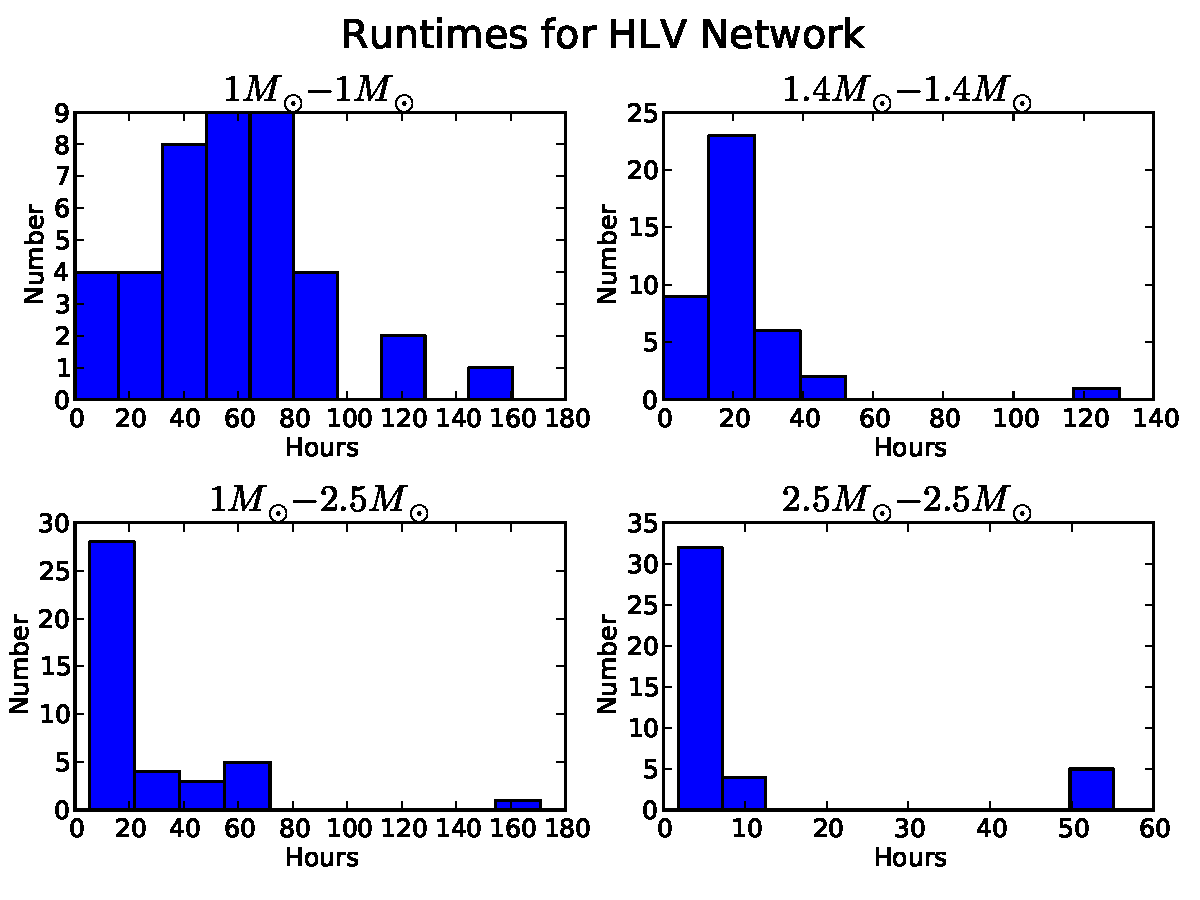
\includegraphics[trim=0cm 0cm 0cm 0cm, clip=true,scale=0.65]{HLVRuntimes.pdf}
 \label{HLVRuntimes}
 \caption{Typical Runtimes for the HLV Network Configuration.  Each run was done on the local Northwestern supercomputer}
\end{figure*}

\begin{figure*}[h!]
  \centering
 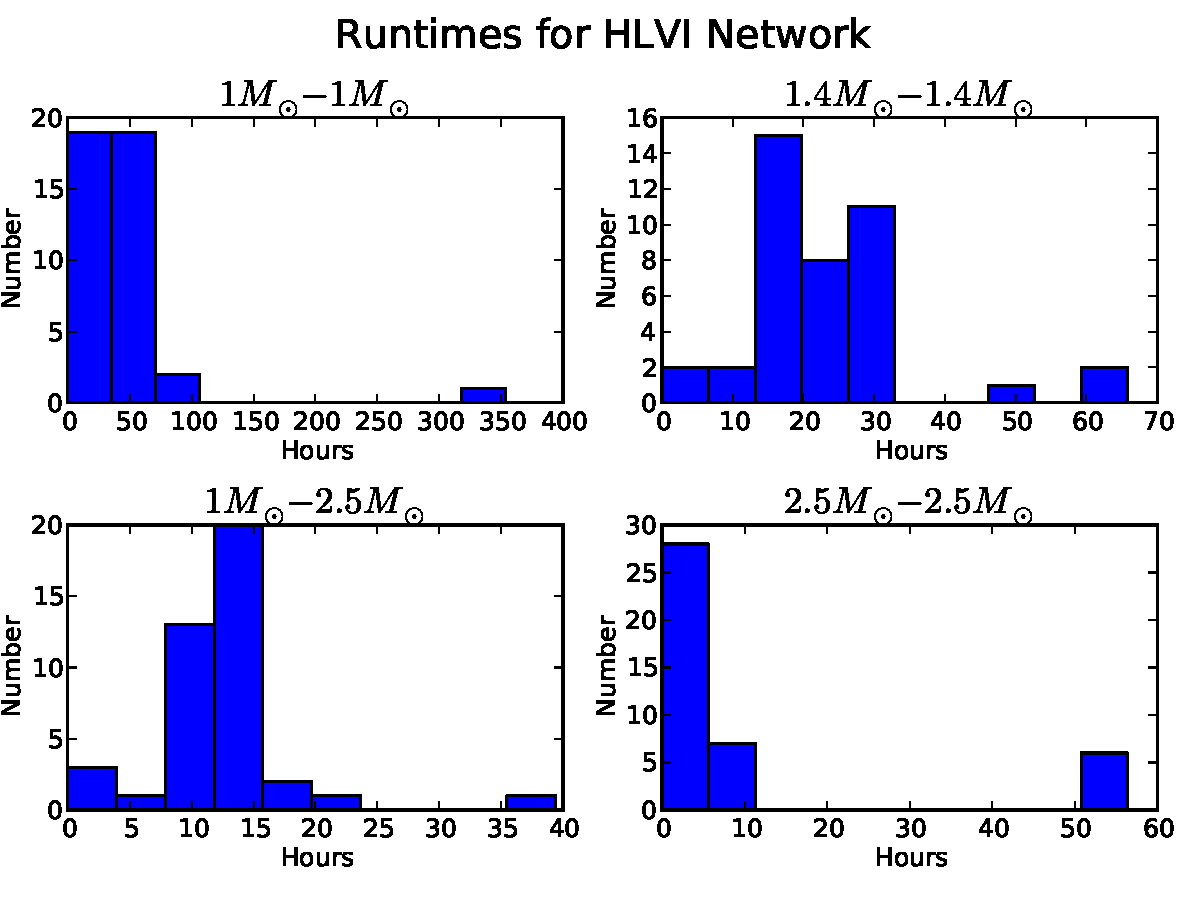
\includegraphics[trim=0cm 0cm 0cm 0cm, clip=true,scale=0.65]{HLVIRuntimes.pdf}
 \label{HLVIRuntimes}
 \caption{\carl{this is superfluous; combine this into one figure with two colors.} }
\end{figure*}

The parameter estimation techniques described here will be performed as a follow-up analysis
to the detections returned by various on-line analyses in the Advanced LIGO/Virgo era.  While
there exist specific PE analyses that will be performed in real-time for time sensitive signals 
(i.e. extrinsic parameters for signals with a potential optimal counterpart \carl{[CITE PROTO-BEN
OR LEO SINGER]}), most PE will require several days to weeks to complete the analysis upon a 
single event.  We display the distribution of runtimes for the two network configuration in Figures~\ref{HLVRuntimes} and ~\ref{HLVIRuntimes} 
\end{comment}

\section{Credible Intervals}
\label{ciSection}

When quoting parameter estimation results, it is often convenient to reduce the full parameter space to
credible intervals about single, marginalized parameters..  To that end, we state the averaged 65\% 
confidence intervals about the single parameters for each of the three parameter pairs of interest.  These were already
 plotted for the sky locations in Figures~\ref{2525SkyLocHLV} and \ref{2525SkyLocHLVI}.  

There are several different ways of computing the width of a credible interval in this setup.  If one considers the points in
 the MCMC as random draws from the true posterior, then the $\alpha$-level credible interval can be computed by simply
  ordering the points, removing $N(1-\alpha )/2$ points from both sides of the posterior samples symmetrically, and measuring
   the width of the remaining points.  While this procedure can prove hazardous for multi-modal distributions, it is 
   straightforward and reliable for single-peaked distributions as reported here.

In Table~\ref{ciTableIntrinsic}, we list the mean 65\% confidence intervals recovered for the four mass configurations in both 
network configurations. This essentially quantifies the widths of the posteriors plotted throughout Section~\ref{resultsSection}.
  The purpose of Tables~\ref{ciTableIntrinsic} and \ref{ciTableExtrinsic} is to provide a quantitative and quotable source for studies seeking to determine how 
  well a physical question about BNS systems can be answered with the Advanced LIGO/Virgo network.


\begin{table*}[t!]
\centering
\caption{Mean 65\% confidence intervals for intrinsic parameters for each of the four systems considered.  We report the confidence intervals of quantities measured, as well as the component masses and total mass.  Although the results for the 
HLV and HLVI configurations are quantitatively identical, we report them separately for consistancy.}
\begin{tabular}{lcccccccccc}

\\HLVI\\
\hline\hline
System & \vline &  $\Delta \chmass / \chmass$ & \vline & $\Delta M_1 / M_1$ & \vline & $\Delta M_2 / M_2$ & \vline & $\Delta M_{tot}/M_{tot}$ & \vline & $\Delta q$\\
\hline\hline
$1M_{\odot}-1M_{\odot}$ & \vline & $4.70\times 10^{-5}$ & \vline & $6.83\times 10^{-2}$ & \vline & $6.09\times 10^{-2}$ & \vline & $3.67\times 10^{-3}$ & \vline & $1.17\times 10^{-1}$\\
\hline
$1.4M_{\odot}-1.4M_{\odot}$ & \vline & $8.27\times 10^{-5}$ & \vline & $7.27\times 10^{-2}$ & \vline & $6.45\times 10^{-2}$ & \vline & $4.10\times 10^{-3}$ & \vline & $1.24\times 10^{-1}$ \\
\hline
$1M_{\odot}-2.5M_{\odot}$ & \vline & $1.65\times 10^{-4}$ & \vline & $1.74\times 10^{-2}$ & \vline & $1.49\times 10^{-2}$ & \vline & $8.15\times 10^{-3}$ & \vline & $1.29\times 10^{-2}$\\\hline
$2.5M_{\odot}-2.5M_{\odot}$ & \vline & $2.29\times 10^{-4}$ & \vline & $8.52\times 10^{-2}$ & \vline & $7.41\times 10^{-2}$ & \vline & $5.51\times 10^{-3}$ & \vline & $1.41\times 10^{-1}$\\
\hline\hline

\\
HLV\\

\hline\hline
System & \vline &  $\Delta \chmass / \chmass$ & \vline & $\Delta M_1 / M_1$ & \vline & $\Delta M_2 / M_2$ & \vline & $\Delta M_{tot}/M_{tot}$ & \vline & $\Delta q$\\
\hline\hline
$1M_{\odot}-1M_{\odot}$ & \vline & $4.66\times 10^{-5}$ & \vline & $6.82\times 10^{-2}$ & \vline & $6.09\times 10^{-2}$ & \vline & $3.64\times 10^{-3}$ & \vline & $1.17\times 10^{-1}$ \\
\hline
$1.4M_{\odot}-1.4M_{\odot}$ & \vline & $8.31\times 10^{-5}$ & \vline & $7.35\times 10^{-2}$ & \vline & $6.51\times 10^{-2}$ & \vline & $4.18\times 10^{-3}$ & \vline & $1.25\times 10^{-1}$\\
\hline
$1M_{\odot}-2.5M_{\odot}$ & \vline & $1.65\times 10^{-4}$ & \vline & $1.75\times 10^{-2}$ & \vline & $1.50\times 10^{-2}$ & \vline & $8.19\times 10^{-3}$ & \vline & $1.30\times 10^{-2}$ \\
\hline
$2.5M_{\odot}-2.5M_{\odot}$ & \vline & $2.30\times 10^{-4}$ & \vline & $8.53\times 10^{-2}$ & \vline & $7.42\times 10^{-2}$ & \vline & $5.52\times 10^{-3}$ & \vline & $1.41\times 10^{-1}$ \\
\hline\hline


\end{tabular}
\label{ciTableIntrinsic}
\end{table*}

 
\begin{table*}[t!]
\centering
\caption{Mean 65\% confidence intervals of extrinsic parameters for each of the four systems considered.  As expected,
there exists a substantial improvement in the sky localization capabilities of the four-detector HLVI configuration over
the three-detector HLV configuration.  Note that the solid-angle sky-location confidence intervals, $\Delta\Omega$, are 
calculated directly on the 2D sphere, not by combining the $\alpha$ and $\delta$ uncertainties.}
\begin{tabular}{lcccccccccc}

\\HLVI\\
\hline\hline
 System & \vline & $\Delta D$ $(mpc)$ & \vline & $\Delta |\cos(\iota)|$ & \vline & $\Delta \alpha$ $(deg)$& \vline &  $\Delta \delta$   $(deg)$ & \vline & $\Delta\Omega$ $(deg^2)$\\
\hline\hline
 $1M_{\odot}-1M_{\odot}$ & \vline & $3.64\times 10^{1}$ & \vline & $2.23\times 10^{-1}$ & \vline & $1.45$ & \vline & $1.48$ & \vline & $1.88$\\
\hline
 $1.4M_{\odot}-1.4M_{\odot}$ & \vline & $5.52\times 10^{1}$ & \vline & $2.56\times 10^{-1}$ & \vline & $1.49$ & \vline & $1.50$ & \vline & $2.26$\\
\hline
 $1M_{\odot}-2.5M_{\odot}$  & \vline & $6.48\times 10^{1}$ & \vline & $2.93\times 10^{-1}$ & \vline & $1.54$ & \vline & $1.64$ & \vline & $2.10$\\
 \hline
 $2.5M_{\odot}-2.5M_{\odot}$ & \vline & $1.06\times 10^{2}$ & \vline & $2.99\times 10^{-1}$ & \vline & $1.03\times 10^{1}$ & \vline & $1.61$ & \vline & $2.22$\\
\hline\hline

\\
HLV\\

\hline\hline
 System & \vline & $\Delta D$ $(mpc)$ & \vline & $\Delta |\cos(\iota)|$ & \vline & $\Delta \alpha$ $(deg)$& \vline &  $\Delta \delta$   $(deg)$ & \vline & $\Delta\Omega$ $(deg^2)$\\
\hline\hline
 $1M_{\odot}-1M_{\odot}$ & \vline & $4.34\times 10^{1}$ & \vline & $3.04\times 10^{-1}$ & \vline & $1.45\times 10^{1}$ & \vline & $6.24$ & \vline & $5.57$\\
\hline
 $1.4M_{\odot}-1.4M_{\odot}$  & \vline & $5.32\times 10^{1}$ & \vline & $2.87\times 10^{-1}$ & \vline & $6.92$ & \vline & $7.11$ & \vline & $8.35$\\
\hline
  $1M_{\odot}-2.5M_{\odot}$& \vline & $6.11\times 10^{1}$ & \vline & $3.11\times 10^{-1}$ & \vline & $2.67$ & \vline & $4.20$ & \vline & $7.39$\\
\hline
 $2.5M_{\odot}-2.5M_{\odot}$ & \vline & $1.04\times 10^{2}$ & \vline & $3.42\times 10^{-1}$ & \vline & $1.13\times 10^{1}$ & \vline & $3.31$ & \vline & $6.27$\\
\hline\hline


\end{tabular}
\label{ciTableExtrinsic}
\end{table*}


\section{Conclusion}
\label{conclusionSection}

In this paper, we performed an MCMC parameter estimation analysis on the recoverability of basic information about binary 
neutron stars, using two projected versions of the Advanced LIGO/Virgo network.  We focused on the recovery of the two 
masses, the luminosity distance, orbital inclination, and the sky location, as these are the six basic parameters of physical 
interest to the problem.  We found that, neglecting the effects of spin, the component masses can be constrained to within
 10\% of their true value to a confidence of 65\%.  This value drops below 2\% for systems with an asymmetric mass ratio.
 These results were summarized in Table \ref{ciTableIntrinsic}.
 
We also reported on the ability of the two network configurations to constrain the
luminosity distance and orbital inclination.  For distance, it was found that the uncertainties
will fall anywhere from 40 to 100 MPC at 65\% confidence, making the uncertainties frequently larger than the luminosity
distances themselves.  However, it was found that the cosine of the orbital inclination can be constrained to within 
0.3 at the 65\% level, suggesting that Advanced LIGO/Virgo will be able to offer some information on GRB beaming
angles in coincidence with electromagnetic observations.

Finally, we reported the ability of advanced networks to constrain the sky location of BNS signals.  It was found that 
the three-detector configuration, consisting of the Washington and Louisiana LIGO sites plus the Italian Virgo site,
 was able to constrain all signals within 60 $deg^2$ on the sky at the 65\% confidence interval, with an average
65\% confidence interval of $\sim 7$ $deg^2$.  Meanwhile, the four-detector
configuration, consisting of the three-detector sites plus a LIGO India detector, was able to localize the sky-locations
to within  13 $deg^2$ on the sky at the 65\% confidence interval, with an average
65\% confidence interval of $\sim 2$ $deg^2$.

It should be noted that there are two distinct types of systematic error, highly relevant to the gravitational-wave parameter estimation problem, that we have not addressed in this study.  First, we have studied the parameter estimation uncertainties under the assumption that the waveform template we use to recover the signal template exactly matches the fully relativistic waveforms nature provides.  In practice, these waveforms are only approximations to the fully general-relativistic physics required to solve the problem.  See \carl{[CITE]} for a better description of the systematic uncertainties present in the most common waveform families.  Additionally, there are several astrophysical assumptions that can potentially contribute
to systematic uncertainties in the waveforms, such as the neutron-star equation of state, possible modifications to 
General Relativity, eccentricity, etc.

Secondly, as stated above, the noise realization that we have employed here is an substantial idealization.  In practice the noise levels of Advanced LIGO and Advanced Virgo will be highly variable over time, and will \emph{not} be stationary or Gaussian, as is commonly assumed.  Unfortunately, there is no reliable or simple way to simulate the sort of non-Gaussian detector glitches and instrumentation effects that will arise in any advanced gravitational-wave detector.  Since the realization of noise will be the primary factor in the deflection of true signal PDFs from the averages quoted here \carl{[TYSON WILL WRITE]}

In this study, we have also neglected the effects of spin in the parameter space, electing to focus on the absolute basic
 parameters that will be measured routinely in the Advanced Detector era.  Given the high degree of coupling
between the spin and the mass of objects in the gravitational-wave parameter space, it remains unclear
if the mass measurement alone will be sufficient to distinguish non-spinning neutron stars from highly-spinning low-mass
black holes.  Future work will explore this potential mass/spin degeneracy, including the effects of orbital precession, with the aim of definitively answering this question.  

\carl{
\section{TODO}
 \begin{itemize}
 \item Finish adding bibliography/sources
 \item double check the distribution of sources in Distance/Iota; make sure iota is actually uniform in cos(i)
 \end{itemize}
 }

\bibliographystyle{apj}
\bibliography{paper}{}

\end{document}
